%%%%%%%%%%%%%%%%%%%%%%%%%%%%%%%%%%%%%%%%
% datoteka.tex
%



\documentclass[a4paper, 12pt]{book}
%\documentclass[a4paper, 12pt, draft]{book}  Nalogo preverite tudi z opcijo draft, ki vam bo pokazala, katere vrstice so predolge!



\usepackage[utf8x]{inputenc}   % omogoča uporabo slovenskih črk kodiranih v formatu UTF-8
\usepackage[slovene,english]{babel}    % naloži, med drugim, slovenske delilne vzorce
\usepackage[pdftex]{graphicx}  % omogoča vlaganje slik različnih formatov
\usepackage{fancyhdr}          % poskrbi, na primer, za glave strani
\usepackage{amssymb}           % dodatni simboli
\usepackage{amsmath}           % eqref, npr.
%\usepackage{hyperxmp}
\usepackage[hyphens]{url}  % dodal Solina
\usepackage{comment}       % dodal Solina

\usepackage[pdftex, colorlinks=true,
						citecolor=black, filecolor=black, 
						linkcolor=black, urlcolor=black,
						pagebackref=false, 
						pdfproducer={LaTeX}, pdfcreator={LaTeX}, hidelinks]{hyperref}

\usepackage{color}       % dodal Solina
\usepackage{soul}       % dodal Solina


%%%%%%%%%%%%%%%%%%%%%%%%%%%%%%%%%%%%%%%%
%	CUSTOME
%%%%%%%%%%%%%%%%%%%%%%%%%%%%%%%%%%%%%%%%
\usepackage{array}
\usepackage{tabularx}
\usepackage{listings}
\usepackage{xcolor}


\renewcommand{\lstlistingname}{Koda}
\renewcommand{\lstlistlistingname}{Seznam kod}

\newcolumntype{b}{X}
\newcolumntype{s}{>{\hsize=.9\hsize}X}
\newcolumntype{z}{>{\hsize=.2\hsize}X}

\definecolor{codegreen}{rgb}{0,0.6,0}
\definecolor{codegray}{rgb}{0.5,0.5,0.5}
\definecolor{codepurple}{rgb}{0.20,0,0.82}
\definecolor{backcolour}{rgb}{0.97,0.97,0.97}

\lstdefinestyle{mystyle}{
    backgroundcolor=\color{backcolour},   
    commentstyle=\color{codegreen},
    keywordstyle=\color{magenta},
    numberstyle=\tiny\color{codegray},
    stringstyle=\color{codepurple},
    basicstyle=\ttfamily\footnotesize,
    breakatwhitespace=false,         
    breaklines=true,                 
    captionpos=b,                    
    keepspaces=true,                 
    numbers=left,                    
    numbersep=5pt,                  
    showspaces=false,                
    showstringspaces=false,
    showtabs=false,                  
    tabsize=2
}

%%%%%%%%%%%%%%%%%%%%%%%%%%%%%%%%%%%%%%%%
%	DIPLOMA INFO
%%%%%%%%%%%%%%%%%%%%%%%%%%%%%%%%%%%%%%%%
\newcommand{\ttitle}{Spletni portal - Urejanje in pregled raziskovalnih objav s področja hrane}
\newcommand{\ttitleEn}{Web Portal -  Reviewing and managing publications of food research }
\newcommand{\tsubject}{\ttitle}
\newcommand{\tsubjectEn}{\ttitleEn}
\newcommand{\tauthor}{Žiga Marolt}
\newcommand{\tkeywords}{spletna aplikcija, go, mikrostoritev, docker, open-api, spletni vmestnik, postgresql, css, html, tailwind, cqrs}
\newcommand{\tkeywordsEn}{big data, database comparison, web application, golang, microservice, docker, open api}


%%%%%%%%%%%%%%%%%%%%%%%%%%%%%%%%%%%%%%%%
%	HYPERREF SETUP
%%%%%%%%%%%%%%%%%%%%%%%%%%%%%%%%%%%%%%%%
\hypersetup{pdftitle={\ttitle}}
\hypersetup{pdfsubject=\ttitleEn}
\hypersetup{pdfauthor={\tauthor, zm1218@student.uni-lj.si}}
\hypersetup{pdfkeywords=\tkeywordsEn}


%%%%%%%%%%%%%%%%%%%%%%%%%%%%%%%%%%%%%%%%
% postavitev strani
%%%%%%%%%%%%%%%%%%%%%%%%%%%%%%%%%%%%%%%%  

\addtolength{\marginparwidth}{-20pt} % robovi za tisk
\addtolength{\oddsidemargin}{40pt}
\addtolength{\evensidemargin}{-40pt}

\renewcommand{\baselinestretch}{1.3} % ustrezen razmik med vrsticami
\setlength{\headheight}{15pt}        % potreben prostor na vrhu
\renewcommand{\chaptermark}[1]%
{\markboth{\MakeUppercase{\thechapter.\ #1}}{}} \renewcommand{\sectionmark}[1]%
{\markright{\MakeUppercase{\thesection.\ #1}}} \renewcommand{\headrulewidth}{0.5pt} \renewcommand{\footrulewidth}{0pt}
\fancyhf{}
\fancyhead[LE,RO]{\sl \thepage} 
\fancyhead[LO]{\sl \rightmark} \fancyhead[RE]{\sl \leftmark}
% \fancyhead[RE]{\sc \tauthor}              % dodal Solina
% \fancyhead[LO]{\sc Diplomska naloga}     % dodal Solina


\newcommand{\BibTeX}{{\sc Bib}\TeX}

%%%%%%%%%%%%%%%%%%%%%%%%%%%%%%%%%%%%%%%%
% naslovi
%%%%%%%%%%%%%%%%%%%%%%%%%%%%%%%%%%%%%%%%  


\newcommand{\autfont}{\Large}
\newcommand{\titfont}{\LARGE\bf}
\newcommand{\clearemptydoublepage}{\newpage{\pagestyle{empty}\cleardoublepage}}
\setcounter{tocdepth}{1}	      % globina kazala

%%%%%%%%%%%%%%%%%%%%%%%%%%%%%%%%%%%%%%%%
% konstrukti
%%%%%%%%%%%%%%%%%%%%%%%%%%%%%%%%%%%%%%%%  
\newtheorem{izrek}{Izrek}[chapter]
\newtheorem{trditev}{Trditev}[izrek]
\newenvironment{dokaz}{\emph{Dokaz.}\ }{\hspace{\fill}{$\Box$}}

%%%%%%%%%%%%%%%%%%%%%%%%%%%%%%%%%%%%%%%%%%%%%%%%%%%%%%%%%%%%%%%%%%%%%%%%%%%%%%%
%% PDF-A
%%%%%%%%%%%%%%%%%%%%%%%%%%%%%%%%%%%%%%%%%%%%%%%%%%%%%%%%%%%%%%%%%%%%%%%%%%%%%%%


%%%%%%%%%%%%%%%%%%%%%%%%%%%%%%%%%%%%%%%% 
% define medatata
%%%%%%%%%%%%%%%%%%%%%%%%%%%%%%%%%%%%%%%% 
\def\Title{\ttitle}
\def\Author{\tauthor, zm1218@student.uni-lj.si}
\def\Subject{\ttitleEn}
\def\Keywords{\tkeywordsEn}

%%%%%%%%%%%%%%%%%%%%%%%%%%%%%%%%%%%%%%%% 
% \convertDate converts D:20080419103507+02'00' to 2008-04-19T10:35:07+02:00
%%%%%%%%%%%%%%%%%%%%%%%%%%%%%%%%%%%%%%%% 
\def\convertDate{%
    \getYear
}

{\catcode`\D=12
 \gdef\getYear D:#1#2#3#4{\edef\xYear{#1#2#3#4}\getMonth}
}
\def\getMonth#1#2{\edef\xMonth{#1#2}\getDay}
\def\getDay#1#2{\edef\xDay{#1#2}\getHour}
\def\getHour#1#2{\edef\xHour{#1#2}\getMin}
\def\getMin#1#2{\edef\xMin{#1#2}\getSec}
\def\getSec#1#2{\edef\xSec{#1#2}\getTZh}
\def\getTZh +#1#2{\edef\xTZh{#1#2}\getTZm}
\def\getTZm '#1#2'{%
    \edef\xTZm{#1#2}%
    \edef\convDate{\xYear-\xMonth-\xDay T\xHour:\xMin:\xSec+\xTZh:\xTZm}%
}

\expandafter\convertDate\pdfcreationdate 

%%%%%%%%%%%%%%%%%%%%%%%%%%%%%%%%%%%%%%%%
% get pdftex version string
%%%%%%%%%%%%%%%%%%%%%%%%%%%%%%%%%%%%%%%% 
\newcount\countA
\countA=\pdftexversion
\advance \countA by -100
\def\pdftexVersionStr{pdfTeX-1.\the\countA.\pdftexrevision}


%%%%%%%%%%%%%%%%%%%%%%%%%%%%%%%%%%%%%%%%
% XMP data
%%%%%%%%%%%%%%%%%%%%%%%%%%%%%%%%%%%%%%%%  
\usepackage{xmpincl}

%%%%%%%%%%%%%%%%%%%%%%%%%%%%%%%%%%%%%%%%
% pdfInfo
%%%%%%%%%%%%%%%%%%%%%%%%%%%%%%%%%%%%%%%%  
\pdfinfo{%
    /Title    (\ttitle)
    /Author   (\tauthor, zm1218@student.uni-lj.si)
    /Subject  (\ttitleEn)
    /Keywords (\tkeywordsEn)
    /ModDate  (\pdfcreationdate)
    /Trapped  /False
}

% list

\newenvironment{myitemize}
{ \begin{itemize}
    \setlength{\itemsep}{2pt}
    \setlength{\parskip}{0pt}
    \setlength{\parsep}{2pt}     }
{ \end{itemize}                  } 


%%%%%%%%%%%%%%%%%%%%%%%%%%%%%%%%%%%%%%%%%%%%%%%%%%%%%%%%%%%%%%%%%%%%%%%%%%%%%%%
%%%%%%%%%%%%%%%%%%%%%%%%%%%%%%%%%%%%%%%%%%%%%%%%%%%%%%%%%%%%%%%%%%%%%%%%%%%%%%%
\begin{document}
\selectlanguage{slovene}
\frontmatter
\setcounter{page}{1} %
\renewcommand{\thepage}{}       % preprecimo težave s številkami strani v kazalu
\newcommand{\sn}[1]{"`#1"'}                    % dodal Solina (slovenski narekovaji)

%%%%%%%%%%%%%%%%%%%%%%%%%%%%%%%%%%%%%%%%
%naslovnica
 \thispagestyle{empty}%
   \begin{center}
    {\large\sc Univerza v Ljubljani\\%
      Fakulteta za računalništvo in informatiko}%
    \vskip 10em%
    {\autfont \tauthor\par}%
    {\titfont \ttitle \par}%
    {\vskip 3em \textsc{DIPLOMSKO DELO\\[5mm]       
    VISOKOŠOLSKI STROKOVNI ŠTUDIJSKI PROGRAM\\ PRVE STOPNJE\\ RAČUNALNIŠTVO IN INFORMATIKA}\par}%
    \vfill\null%
    {\large \textsc{Mentor}: doc.\ dr.  Mira Trebar\par}%
    {\vskip 2em \large Ljubljana, 2021 \par}%
\end{center}
% prazna stran
%\clearemptydoublepage      % dodal Solina (izjava o licencah itd. se izpiše na hrbtni strani naslovnice)

%%%%%%%%%%%%%%%%%%%%%%%%%%%%%%%%%%%%%%%%
%copyright stran
\thispagestyle{empty}
\vspace*{8cm}

\noindent
{\sc Copyright}. 
Rezultati diplomske naloge so intelektualna lastnina avtorja in Fakultete za računalništvo in informatiko Univerze v Ljubljani.
Za objavo in koriščenje rezultatov diplomske naloge je potrebno pisno privoljenje avtorja, Fakultete za računalništvo in informatiko ter mentorja.

\begin{center}
\mbox{}\vfill
\emph{Besedilo je oblikovano z urejevalnikom besedil \LaTeX.}
\end{center}
% prazna stran
\clearemptydoublepage

%%%%%%%%%%%%%%%%%%%%%%%%%%%%%%%%%%%%%%%%
% stran 3 med uvodnimi listi
\thispagestyle{empty}
\vspace*{4cm}

\noindent
Fakulteta za računalništvo in informatiko izdaja naslednjo nalogo:
\medskip
\begin{tabbing}
\hspace{32mm}\= \hspace{6cm} \= \kill




Tematika naloge:
\end{tabbing}

Spletna aplikacija za pregled raziskovalnih metod s področja analize in napovedovanja dobe
uporabnosti hitro pokvarljivih živil, kot sta sveže meso in ribe.
V aplikaciji se uporablja pristop vodenja evidenc.  Ta metoda kot vir podatkov uporablja že obstoječe
zanesljive dokumente in podobne vire informacij za zbiranje podatkov. Na osnovi vnaprej definiranih
živil se za izbrano živilo nahajajo podatki, ki omogočajo pregled zahtev v hladni verigi, raziskovalnih
metod, raziskovalcev, inštitucij, raziskovalnih laboratorijev, objavljenih člankov, podatkovnih baz,
programskih orodij,  …

Obseg naloge in podrobnejši opis bi definirali v nadaljevanju. Pomembno je, da bi zasnovali ustrezen
model podatkovne baze tako, da lahko v aplikaciji  prijavljen uporabnik dodaja vsebine za neko živilo.
Pred objavo, pa jih mora potrditi odgovorna oseba. Zasnovana mora biti tako, da je možno do nje
dostopati iz poljubne aplikacije. Testiranje bi izvedli z enostavnim spletnim portalom, kjer bi vnesli
testne podatke iz nekaj raziskovalnih člankov.

\vspace{15mm}






\vspace{2cm}

% prazna stran
\clearemptydoublepage

% zahvala
\thispagestyle{empty}\mbox{}\vfill\null\it%
\noindent
Zahvaljujem se mentorici doc. dr. Miri Trebar za vso pomoč in druzini za podporo.
\rm\normalfont

% prazna stran
\clearemptydoublepage


%%%%%%%%%%%%%%%%%%%%%%%%%%%%%%%%%%%%%%%%
% kazalo
\pagestyle{empty}
\def\thepage{}% preprecimo tezave s stevilkami strani v kazalu
\tableofcontents{}


% tole naj bi mi kao clearalo empty page pa mi ne !
\let\cleardoublepage=\clearpage

%%%%%%%%%%%%%%%%%%%%%%%%%%%%%%%%%%%%%%%%
% seznam kratic

\chapter*{Seznam uporabljenih kratic}  % spremenil Solina, da predolge vrstice ne gredo preko desnega roba
\noindent\begin{tabular}{p{0.2\textwidth}|p{.35\textwidth}|p{.35\textwidth}}    % po potrebi razširi prvo kolono tabele na račun drugih dveh!
  {\bf kratica} & {\bf angleško}                             & {\bf slovensko} \\ \hline
  {\bf API} & Application Programming Interface & aplikacijski programski vmesnik \\
  {\bf IAAA} & Identification, Authentication, Authorization and Accounting & varnostni koncepti: identifikacija, avtentikacija, avtorizacija in odgovornost \\
  {\bf CSS} & Cascading Style Sheets & predloge, ki določajo izgled spletnih strani \\
  {\bf ER diagram} & Entity Relationship Diagram & entitetno relacijski diagram \\
  {\bf HTML} & Hyper Text Markup Language & označevalni jezik za izdelavo spletnih strani \\
  {\bf HTTP} & Hyper Text Transfer Protocol & komunikacijski spletni protokol \\
  {\bf JSON} & JavaScript Object Notation & objektna notacija za JavaScript \\
  {\bf oktet} byte & Digitalna enota, ki predstavlja osem bitov \\
%   {\bf PDF} & Portable Document Format & format prenosnega dokumenta \\
  {\bf REST} & Representational state transfer & predstavitveni prenos stanja \\
  {\bf SQL} & Structured Query Language & strukturiran poizvedovalni jezik \\
  {\bf URL} & Uniform Resource Locator & enolični krajevnik vira \\
%  \dots & \dots & \dots \\
\end{tabular}


% prazna stran
\clearemptydoublepage

%%%%%%%%%%%%%%%%%%%%%%%%%%%%%%%%%%%%%%%%
% povzetek
\addcontentsline{toc}{chapter}{Povzetek}
\chapter*{Povzetek}

\noindent\textbf{Naslov:} \ttitle
\bigskip

\noindent\textbf{Avtor:} \tauthor
\bigskip

%\noindent\textbf{Povzetek:} 
\noindent
V sobodni informacijski druzbi je veliko podatkov in ogromno podatkov, ki nas ne zanimajo. Da pridemo do podatkov, ki jih zelimo, uporabimo razlicne filtre, ki jih izvedemo nad obstojecimi podatki. Vendar pa je vcasih teh podatkov prevec in iskanje traja predolgo.

Naloga te diplomske naloge je raziskati in dokazati najbolj primerno podatkovno strukturo, za pregled raziskovalnih metod s področja analize in napovedovanja dobe uporabnosti hitro pokvarljivih živil, kot sta sveže meso in ribe. 

V diplomski nalogi je opisan postopek izdelave spletne aplikacije za vnasanje in iskanje živil. Aplikacija je zasnovana kot mikrostoritev, za razvojno okolje je uporabljena docker arhitektura, kar nam omogoca enostavno postavitev projekta, in pa tudi enostavno objavljanje projekta na pravem okolju. 

V aplikaciji so definirani trije nivoji uporabnikov, ki imajo razlicne dostope do posameznih delov aplikacije. 
\bigskip

\noindent\textbf{Ključne besede:} \tkeywords.
% prazna stran
\clearemptydoublepage

%%%%%%%%%%%%%%%%%%%%%%%%%%%%%%%%%%%%%%%%
% abstract
\selectlanguage{english}
\addcontentsline{toc}{chapter}{Abstract}
\chapter*{Abstract}

\noindent\textbf{Title:} \ttitleEn
\bigskip

\noindent\textbf{Author:} \tauthor
\bigskip

%\noindent\textbf{Abstract:} 
\noindent
Uvod v anglescini
\bigskip

\noindent\textbf{Keywords:} \tkeywordsEn.
\selectlanguage{slovene}
% prazna stran
\clearemptydoublepage

%%%%%%%%%%%%%%%%%%%%%%%%%%%%%%%%%%%%%%%%
\mainmatter
\setcounter{page}{1}
\pagestyle{fancy}

\chapter{Uvod}

V sobodni informacijski družbi je veliko podatkov in ogromno podatkov, ki nas ne zanimajo. Da pridemo do le tistih, ki jih nas interesirajo, uporabimo različne filtre, ki jih izvedemo nad obstoječimi podatki. Vendar pa je vcasih teh podatkov prevec in iskanje traja predolgo.

Naloga te diplomske naloge je raziskati in implementirati najbolj primerno podatkovno strukturo, za pregled raziskovalnih metod s področja analize in napovedovanja dobe uporabnosti hitro pokvarljivih živil, kot sta sveže meso in ribe. 

V diplomski nalogi je opisan postopek izdelave spletne aplikacije za vnasanje in iskanje živil. Aplikacija je zasnovana kot mikrostoritev, za razvojno okolje je uporabljena docker arhitektura, kar nam omogoca enostavno postavitev projekta, in pa tudi enostavno objavljanje projekta na pravem okolju. 

V aplikaciji so definirani trije nivoji uporabnikov, ki imajo razlicne dostope do posameznih delov aplikacije.

Skozi diplomsko nalogo bomo spoznali, najprej kako smo pristopili k reševanju omenjenega problema, kakšen je bil proces dela in sam razvoj končnega izdelka. Na koncu pa bomo spoznali še končno rešitev in samo implementacijo.

\pagebreak

\section{Motivacija}

Iz dneva v dan nam je na voljo vedno več objavljenih raziskav iz področja hrane. Raziskave so objavljene na različnih virih, naj si bo to članek na svetovnem spletu, v reviji ali pa v znanstveni knjigi. Raziskovalci, ki prebirajo raziskave, imajo oteženo delo, poiskati zanesljive vire in iz njih izluščiti pravilne in informativne informacije.

Ker se struktura podatkov razlikuje od raziskave do reziskave, od vira do vira, je pomembno da pravilno definiramo podatkovno strukturo. Za dobro uporabniško izkušnjo mora biti vnos podatkov o raziskavah enostaven in dosleden, iskanje po le teh pa mora biti hitro in uporabno.

Priznajmo si, večina spletnih aplikacij ne rešuje težkih tehničnih izzivov. Pomembno je, da z izdelkom pridemo na trg pred našo konkurenco, zato pa je pomembno, da je izdelek pravilno tehnično strukturiran.
Morda se to sprva sliši dolgočasno, vendar sam mislim, da je podpirati ta cilj težje, kot se sliši.

Med razvojem te aplikacije, ki vam jo bom opisal skozi celotno delo, sem se hotel naučiti čim več. Spoznal sem nov programski jezik - \verb=Go= in nov arhitekturni koncept mikro storitev (angl. microservice). Omenjeni dve stvari sta me dodatno spodbudilo k delu in spoznavanju novih stvari na področju razvoja programse opreme in pa tudi same organizacije.


\chapter{Pregled področja}
\label{pregled-podrocja}
Rok uporabnosti živila je pomembna oznaka vsakega živila. Podaja nam informacijo, koliko časa lahko neko živilo hranimo, da varnost in kakovost izdelka ostaneta v sprejemljivem območju. Ob tem morajo biti upoštevani specifični pogoji transporta in shranjevanja. Določitev roka uporabnosti živila temelji na predpostavki, da z živilom ustrezno ravnamo.

Zamrzovanje živil je eden izmed načinov podaljševanja roka uporabnosti živil. Zamrzniti je mogoče skoraj vsa živila z redkimi izjemami, vendar se je treba zavedati, da kakovost vseh živil po zamrzovanju ni enaka.

Varno uživanje živil zagotavljamo, če upoštevamo rok uporabnosti, poznamo in upoštevamo navodila proizvajalcev za shranjevanje živil, pri hitro pokvarljivih živilih pa vzdržujemo hladno verigo od proizvajalca do končnega uporabnika. Tako zmanjšujemo verjetnost nastanka okužb in zastrupitev, povzročenih z živili, nenazadnje pa tudi na količine živilskih odpadkov.

\textbf{Hladna veriga} je vzdrževanje predpisane, dovolj nizke, temperature živila, s ciljem ohranitve čim boljše kakovosti in varnosti živila v celotni živilski verigi, od proizvodnje, transporta, 
shranjevanja in distribucije do porabe pri končnem potrošniku. 
Običajno je to temperatura 4−8 °C, pri kateri se razvoj mikroorganizmov upočasni. Priporočena temperatura je predpisana na označbi izdelka. \cite{nijz-brosura-varnost}

V tabeli spodaj \ref{tab:food-safety-table} navajamo orientacijske vrednosti okvirnega roka uporabnosti takega živila.

\begin{table}[h]
\begin{tabular}{lll}
\textbf{Predelano živilo} & \textbf{Neodprto, po nakupu} & \textbf{Po odprtju}        \\
Kuhana perutnina          & 3 do 4 dni                   & 3 do 4 dni                 \\
Kuhane klobase            & 3 do 4 dni                   & 3 do 4 dni                 \\
Dimljene klobase          & 6 tednov/shramba             & 3 tedne                    \\
Slanina                   & 2 tedna                      & 7 dni                      \\
Hrenovke                  & 2 tedna                      & 1 teden                    \\
Šunka, kuhana             & 7 dni                        & rezine 3 dni; v kosu,7 dni
\end{tabular}
\caption{ Povzeto po USDA, Food safety and inspection service, 2011 }
\label{tab:food-safety-table}
\end{table}

\section{Pregled zahtev}

Namen aplikacije je, agregirati podatke iz razlčnih virov. Naj bo to knjiga, spletni vir ali pa revija. Vnašanje le teh podatkov iz nedefiniranih virov je težko in zamudno opravilo. Aplikacija mora biti razvita z namenom, da je uporabniku delo olajšano, z v naprej predlaganimi vrednostmi za posamezne podatke. 

Pomembno je, da zasnujemo ustrezen model podatkovne baze tako, da lahko v aplikaciji prijavljen uporabnik dodaja in ureja vsebine za neko živilo ne glede na to iz katerega vira izhajajo podatki. 
Struktura podatkov je lahko različna glede na vire podatkov, zatorej je potrebno razmisliti, kako dodajati in definirati podatke za neko novo vrednost, ki je sistemu še nepoznana.

Aplikacija mora biti pregleda in enostavna za uporabo, uporabniku naj pomaga pri iskanju podatkov, ki so bili vnešeni v podatkovno bazo. Dostop do aplikacije naj bo omogočen le prjavljenim uporabnikom. Posamezne strani pa naj bodo vidne le nekaterim uporabnikom, glede na vlogo ki je dodeljena uporabniku.

\begin{description}
\item[Vloge uporabnikov]:
	\begin{itemize}
		\item \textbf{Uporabnik} - prijavljen uporabnik z uporabniškim imenom in geslom, brez dodatnih pravic
		\item \textbf{Urednik} - prijavljen uporabnik z uporabniškim imenom in geslom, lahko ureja in dodaja vsebine
		\item \textbf{Administrator} - prijavljen uporabnik z uporabniškim imenom in geslomm s polnim nadzorom aplikacije
	\end{itemize}
\end{description}

\section{Pregled obstoječih rešitev}

Najprej smo raziskali trg, in preverili, ali taka rešitev že obstaja na trgu. S tem smo razmislili, ali je problem sploh smislen, in vreden razvoja. Med raziskavo smo odkrili nekaj orodij, ki odpravljajo podobno težavo, vendar nobenega, ki bi popolnoma ustrezal našim zahtevkom. 
Ena izmed orodij, ki smo jo zasledili je "Food Safety Centre" \cite{food-safety-centre}.

% ===================
% RAZVOJ APLIKACIJE
% ===================
\chapter{Razvoj Aplikacije}
\label{razvoj}
V tem sklopu bomo spoznali celoten proces razvoja našega izdelka. Z opisom vpeljanega procesa, bomo spoznali zakaj je pomembno, da na začetku projekta, dobro definiramo komunikacijo in odvisnost med posameznimi storitvami. Spoznali bomo tudi, zakaj smo posvetili čas dokumentiranju aplikacijskega programskega vmestnika in kaj smo s tem pridobili. Opisali bomo posamezne tehnologije, s katerimi je smo se srečali med razvojem aplikacija in čemu je katera tehnologija namenjena. 

\section{Življenjski cikel razvoja }
Življenjski cikel razvoja programske opreme je proces, ki je sestavljen iz vrste načrtovanih dejavnosti za razvoj ali spremembo programskih izdelkov. Vsaka programska oprema pa je zelo specifična, in se razlikuje od problema do problema. Kar pomeni, da je življenski cikel razvoja programske opreme različen od projekta do projekta, zato je potrebno ustrezno izbrati pravi proces, ki omogoča kar se da učinkovit razvoj.

Ustrezen model nam omogoča boljši pregled nas samim procesom razvoja programske opreme in pa tudi testiranje in definiranje le te. Veliko projektov, pri napačni izbiri metodologije prekorači proračun, se prepozno odloči za spreminjane poslovne logike ali pa dostavijo izdelek prepozno. 

Pri razvoju naše aplikacije smo sledili \sn{modelu slapa}, v angleščini poznan kot "Waterfall Model". Omenjena metodologija je linearni model, pri katerem napredek pretežno teče v eno smer navzdol skozi faze zbiranja potreb, analize, načrtovanja, razvoja, testiranja, uvajanja in vzdrževanja. Izraz je bil prvič uveden v dokumentu, ki ga je leta 1970 objavil dr. Winston W. Royce, in se še naprej uporablja v aplikacijah industrijskega oblikovanja. \cite{waterfall-model}

Omenjen model je definiran z zaporedjem različnih faz. Število faz je lahko različno glede na izvedbo metodologije, giblje se med pet in sedem različnimi fazami. Izhod ene faze se uporablja kot vhod naslednje faze, torej mora biti vsaka faza zaključena, preden se lahko začne naslednja faza.

\begin{description}
    \item[Opis posameznih faz]:
    \begin{enumerate}
        \item \textbf{Zbiranje zahtev} – vse možne zahteve so zajete v dokumentih z zahtevami  za izdelek.
        \item \textbf{Analizaranje} - pregled specifikacij in analiziranje le teh. Z analiziranjem se definra poslovno logiko in pa tudi financne plane projekta.
        \item \textbf{Zasnova sistema} - glede na predhodnjo analizo, se načrtuje arhitekturo programske opreme.
        \item \textbf{Izvedba} - Razvoj programske opreme v majhnih enotah s funkcionalnim testiranjem.
        \item \textbf{Integracija in testiranje} - Integracija vsake enote, razvite v prejšnji fazi in po integraciji, testira celoten sistem za morebitne napake.
        \item \textbf{Uvedba sistema} – Po opravljenih vseh funkcionalnih in nefunkcionalnih testiranjih naj izdelek deluje v proizvodnem okolju.
        \item \textbf{Vzdrževanje} - Odpravljanje težav in izdaja nove različice s popravki težav po potrebi.
    \end{enumerate}
\end{description}

Zaradi medsebojne odvisnosti posameznih faz, je model zelo pregleden in jasen pri implementaciji. Vendar ima nekaj pomankljivosti in je učinkovit le pri manjših projektih, kjer zo zahtevki zelo jasno definirani in kjer je predviden obseg dela manjši.
Model ne dovoljuje spreminjanja specifikacij, oziroma je spreminjanje zahtevkov med samo implementacijo oteženo. Ko je izdelek v fazi testiranja, se je težko vrniti in spremeniti nekaj, kar je ostalo v fazi analize.
To pomeni, da delujoč izdelek dobimo šele na koncu cikla omenjenega modela. 

\begin{figure}[h]
\begin{center}
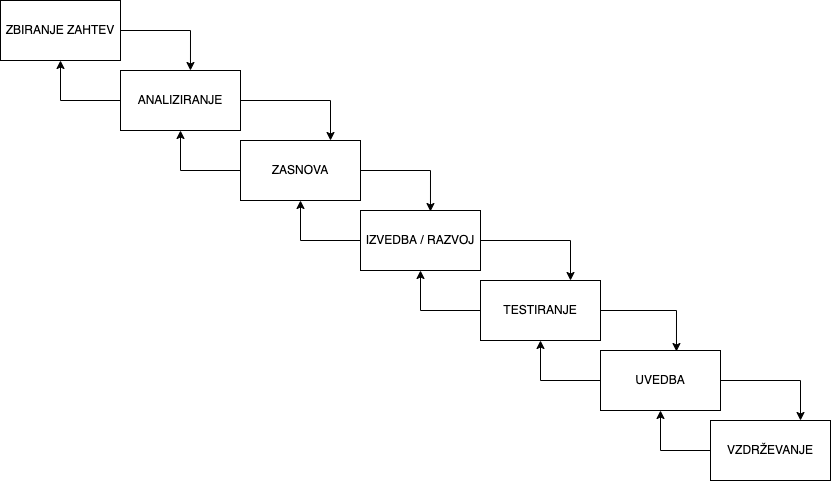
\includegraphics[width=1\textwidth]{slike/waterfall.png}
\end{center}
\caption{ Vizualizacija sedmih faz, prikazanih z grafom }
\label{waterfall-phases}
\end{figure}
\section{Verzioniranje programske kode}

Orodje, ki upravlja in sledi različnim verzijam programske kode ali drugih podatkov, ki so lahko predstavljeni v bitih, je znano kot sistem za verzioniranje podatkov. V angleščini poznamo vec izrazov, ki se navezujejo na omenjeno orodje, to so version control system (VCS), source code manager (SCM), revision control system (RCS) in se nekaj drugih permutacij besed “revision,” “version,” “code,” “content,” “control,” “management,” in “system.”.

Najlažje si je to predstavljati kot, nekakšno podatkovno bazo, ki hrani vse verzije nekih podatkov in nam prikazuje razliko med verzijami. Ponavadi so ti podatki shranjeni nekje na strežniku, da lahko do njih dostopajo vsi, ki delajo z njimi. Torej če delamo spletno stran, lahko tako vidimo kako se spletna stran razvija. Naprimer neka stran ima v verziji v0.1 slepo besedilo (Lorem ipsum), če to primerjamo z verzijo v1.0, kjer je že prava vsebina opazimo spremembo besedila. Shranijo se tudi krajša sporočila, ki omogočajo lažji pregled nad zgodovino sprememb in natančen vpogled kdo je naredil spremembo in kdaj je bila sprememba narejena.
\section{Infrastruktura}
Uporaba programske opreme je zapletena. Pred namestitvijo je potrebno razmisliti, kateri operacijski sistem se bo uporabljal, katera so orodja, ki jih programska oprema potrebuje in še vrsto drugih vprašanj. Večina računalnikov ima že nameščenih in zagnanih več aplikacij. In večina aplikacij je odvisna od druge programske opreme. Kaj se zgodi, če dve ali več aplikacij, ki so nameščene na računalniku, ne delujejo dobro skupaj? Pride do problema, ki pa ga ni tako enostavno odpraviti. Stvari postanejo bolj zapletene, če si aplikacije med sabo delijo skupne vire. 

Na našem projektu smo se hoteli izogniti nevšečnostim z oteženim postavljanjem projekta, zato smo se odločili oporabili orodje za izoliranje okolja. Virtualizacije je postopek, ki strojni ali programski vir preslika v navidezni vir, tega pa potem odjemalec koristi kot pravi vir. Pomembna prednost uporabe virtualizacije je prenostljivost. Z njo lahko dosežemo enake pogoje za izvajanje programske opreme na različnih strojnih opremah, in ravno to si želimo doseči.

V našem projektu smo se odločili uporabili orodje Docker. Orodje nam zagotavlja tako imenovano abstrakcijo, da poenostavljeno delamo z zapletenimi stvarmi in nudi enako okolje vsem uporabnikom, ki delujejo na istem projektu, ne glede na uporabljen operacijski sistem. 

\begin{figure}[h]
\begin{center}
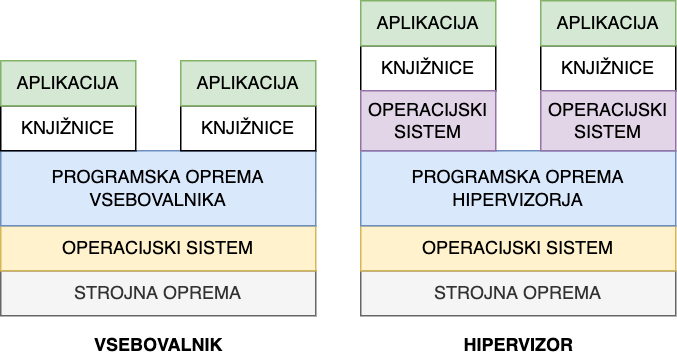
\includegraphics[width=0.75\textwidth]{slike/docker-vs-vm.png}
\end{center}
\caption{ Prikaz razlike med virtualnim strojem in Docker vsebovalnik }
\label{docker-vs-vm}
\end{figure}

\subsection{Docker}
Docker je trenutno najbolj priljubljena rešitev vsebnika. Ponuja številne funkcije in je podprt iz strani ostalih sistemov, kot so naprimer orodja za orkestracijo. V osnovi gre za izolacijo procesov in virtualizacijo virov, do katerih procesi dostopajo. Omogoča izoliranje aplikacije od infrastrukture, za hitro dostavljanje programske opreme. \cite{linuxcontainers} 

Docker je odvisen od jedra Linuxa, kar pomeni, da ne deluje v sistemu Windows ali macOS. V tem primeru je potreben zagon v virtualnem stroju, ki vsebuje jedro $Linuxa$. \cite{docker-in-action}

Konfiguriranje slike vsebnika zahteva ustvarjanje konfiguracijske datoteke, ki je ponavadi znotraj projekta in se imenuje $Dockerfile$. To je tekstovna datoteka, ki opisuje zahteve posameznega programa, kot so osnovna slika za izvajanje (npr. slika ki omogoča izvajanje Go programov), ukazi za zagon (npr. namestitev), vrata, na katerih bo aplikacija poslušala, in tako naprej.

\begin{figure}[h]
\begin{center}
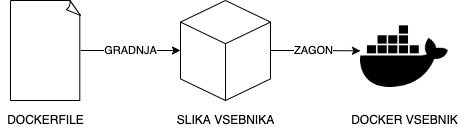
\includegraphics[width=0.75\textwidth]{slike/docker-flow.png}
\end{center}
\caption{ Prikaz gradnje docker vsebovalnikov }
\label{password-reset-form}
\end{figure}

Dockerjeve slike imajo nekakšen sistem odvisnosti. Slika lahko razširi drugo sliko, ki sama lahko razširi še eno. Ko izvaja namestitev, bo Docker prenesel vsako plast in jo predpomnil, tako da bodo naslednje namestitve hitrejše. Da se datotečni sistemi vsake plasti združijo eno na drugo poskrbi sistem UnionFS.  Slike so enote, ki jih je mogoče pošiljati v ekosistemu Docker. Docker ponuja nabor infrastrukturnih komponent, ki poenostavljajo distribucijo slik vmestnikov. Te komponente so registri in indeksi. Na voljo za uporabo je javno dostopno infrastruktura, ki jo nudi $Docker Inc.$, uporabi pa se lahko tudi privatni register, ki ga gostimo sami (naprimer $GitLab$ register).

Vsebniki so skupina procesov v operacijskem sistemu z jedrom Linux, katerim upravlja računske vire z nadzornimi skupinami in zagotavlja izolacijo virov z uporabo imenskih prostorov. Ob zagonu vsebnika se uporabni vsebniška slika (angl. container image) v kateri so zapisane informacije o izvajanju programske opreme in preko katere Docker tudi priklopi nov, prazen bralno-pisalni datotečni sloj. Slika se ustvari s postopkom gradnje, ki je zapisan v datoteki $Dockerfile$. 

V kodi spodaj (\ref{lst:dcb-snipet}), je prikazan primer grajenja slike, ki smo jo uporabili pri razvoju enega zalednega dela naše aplikacije.
\begin{lstlisting}[language=bash, style=mystyle,caption={Grajenje slike docker vmestnika},label=lst:dcb-snipet]
$ docker build .          
[+] Building 69.1s (9/9)                             FINISHED
 => [internal] load build definition from Dockerfile    0.1s
 => => transferring dockerfile: 180B                    0.0s
 => [internal] load .dockerignore                       0.0s
 => => transferring context: 2B                         0.0s
 => [internal] load metadata for golang:1.17            2.7s
 => [1/2] FROM golang:1.17@sha256:39953c7c7             60.0s
 => => resolve golang:1.17@sha256:39953c7c7             0.0s
 => => sha256:0e29546d54 54.92MB / 54.92MB              27.2s
 => => extracting sha256:0e29546d541                    4.5s
 => => sha256:6432567af305a4304605a3 154B / 154B        34.4s
 => [internal] load build context                       0.0s
 => => transferring context: 121B                       0.0s
 => [2/2] COPY start.sh /                               0.0s 
 => exporting to image                                  0.2s 
 => => exporting layers                                 0.2s 
 => => writing image sha256:96d781a9030                 0.0s 
\end{lstlisting}
\section{Arthitektura}
Arhitekturna zasnova močno vpiva na delovanje in razvoj aplikacije. Vsak arhitekturni koncept ima svoje prednosti in slabosti. Na projektu smo hoteli spoznati arhitekturo mikrostoritev. Ta vrsta arhitekture definira aplikacijo, sestavljeno iz majhnih samostojnih enot. Vsaka enota ima točno določeno funkcijo in lahko deluje neodvisno od ostalih enot.

Arhitekturni slog mikrostoritev je pristop k razvoju ene same aplikacije kot zbirke majhnih storitev, od katerih vsaka deluje v svojem procesu in komunicira z enostavnimi mehanizmi, kot je naprimer HTTP API. Te storitve so zgrajene na podlagi poslovnih zmogljivosti in jih je mogoče neodvisno uvesti s popolnoma avtomatiziranimi stroji za uvajanje. Obstaja minimalno centralizirano upravljanje teh storitev, ki so lahko napisane v različnih programskih jezikih in uporabljajo različne tehnologije za shranjevanje podatkov. \cite{mfowler-microservices}

Kot je razvidno na sliki \ref{app-architecture}, smo v naši aplikaciji definirali dve storitvi. Vsaka storitev ima svoja opravila in je neodvosna od ostalih enot. Za medsebojno komunikacijo se uporablja protokol HTTP.

\begin{figure}[h]
\begin{center}
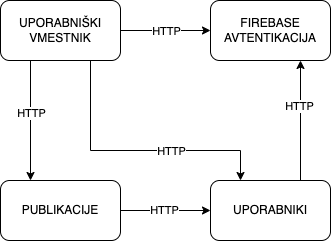
\includegraphics[width=0.75\textwidth]{slike/architecture.png}
\end{center}
\caption{ Arhitektura mikrostoritev naše aplikacije }
\label{app-architecture}
\end{figure}

\newpage
\section{Programski jezik Go}

\verb=Go= (ali golang) je odprtokodni programski jezik, razvit iz strani ameriške kooproracije Google. Pobudniki razvojo so bili Robert Griesemer, Ken Thomson, in Rob Pike. Sprva je bil uporabljen le za interno uporabo, leta 2009 pa so ga ponudili kot odprto kodni programski jezik širši publiki. 
 
Kljub temu, da je programski jezik Go, jezik za splošno uporabo, je njegova primarna uporabna namenjena pisanju sistemskih orodij, spletnih storitev in programov, ki veliko komunicirajo preko  spletnega omrežja. Primeren je tudi za učenje prvega programskega jezika, zaradi njegove enostavnosti in pristopov. Definiranih, oziroma rezerviranih je le 25 ključnih besed, kar pomeni, da si je veliko lažje zapomniti jezik, in se je potrebno naučiti le konceptov.

Čeprav Go ni objektno usmerjen programski jezik, so njegovi vmesniki zelo vsestranski in omogočajo posnemanje nekaterih zmožnosti objektno usmerjenih jezikov, kot so polimorfizem, enkapsulacija in sestava.

Go ima tudi zmožnosti sočasnosti z uporabo preprostega modela sočasnosti, ki se izvaja z uporabo goroutin in kanalov. Go upravlja niti operacijskega sistema namesto nas in ima zmogljiv izvajalni čas. 
To omogoča ustvarjanje lahkih delovnih enot (goroutine), ki med seboj komunicirajo s pomočjo kanalov.
 

 
% \section{Metrike}

% V IT in računalništvu v oblaku je opaznost zmožnost merjenja trenutnega stanja sistema na podlagi podatkov, ki jih ustvari, kot so dnevniki, meritve in sledi.

% Opazovanost je odvisna od telemetrije, ki izhaja iz instrumentov, ki prihajajo iz končnih točk in storitev v vaših računalniških okoljih v več oblakih. V teh sodobnih okoljih vsaka komponenta strojne opreme, programske opreme in infrastrukture v oblaku ter vsak vsebnik, odprtokodno orodje in mikrostoritev ustvari zapise o vsaki dejavnosti. Cilj opazljivosti je razumeti, kaj se dogaja v vseh teh okoljih in med tehnologijami, tako da lahko odkrijete in razrešite težave, da bodo vaši sistemi učinkoviti in zanesljivi, vaše stranke pa zadovoljne.

% Organizacije običajno izvajajo opazljivost s kombinacijo instrumentacijskih metod, vključno z odprtokodnimi instrumentacijskimi orodji, kot je OpenTelemetry.

% Številne organizacije sprejmejo tudi rešitev opazovanja, ki jim pomaga odkriti in analizirati pomen dogodkov za njihovo delovanje, življenjske cikle razvoja programske opreme, varnost aplikacij in izkušnje končnih uporabnikov.

% Opaznost je v zadnjih letih postala bolj kritična, saj so okolja, ki izvirajo iz oblaka, postala bolj zapletena in je vedno težje določiti možne temeljne vzroke za okvaro ali nepravilnost. Ko ekipe začnejo zbirati in delati z opazovanimi podatki, spoznavajo tudi njegove koristi tudi za poslovanje.

% Ker se storitve v oblaku zanašajo na edinstveno porazdeljeno in dinamično arhitekturo, se lahko opaznost včasih nanaša tudi na posebna programska orodja in prakse, ki jih podjetja uporabljajo za razlago podatkov o zmogljivosti v oblaku. Čeprav nekateri ljudje mislijo, da je opaznost modna beseda za prefinjeno spremljanje zmogljivosti aplikacij (APM), je pri primerjavi opaznosti in spremljanja treba upoštevati nekaj ključnih razlik. \cite{ot-what-is-observability}
\section{Spletni strežnik}

Spletni strežnik (angl. Web Server) je računalniški sistem, ki obdeluje zahteve preko protokola \verb=HTTP=. Izraz spletni strežnik se lahko nanaša na celoten sistem ali posebej na programsko opremo, ki sprejema in nadzira zahteve HTTP. Primarna funkcija spletnega strežnika je shranjevanje, obdelava in pošiljanje spletnih strani odjemalcem. Predložene strani so najpogosteje dokumenti HTML, ki poleg besedilne vsebine vključujejo tudi slike, CSS prdloge in skripte. 

Glavna naloga spletnega strežnika je prikazovanje vsebine spletne strani. Če spletni strežnik ni izpostavljen javnosti in se uporablja interno, se imenuje \verb=intranetni strežnik=. Strojna oprema spletnega strežnika je povezana z internetom in omogoča izmenjavo podatkov z drugimi povezanimi napravami, medtem ko programska oprema spletnega strežnika nadzoruje, kako uporabnik dostopa do gostiteljskih datotek.

% Primer spletnega strežnika v programskem jeziku Go (\ref{lst:ws-go}), dosegljivega na naslovu  \url{http://localhost:8080/}.
\begin{lstlisting}[language=go, style=mystyle,caption={Spletni strežnik v programskem jeziku Go},label=lst:ws-go]
package main

import (
    "fmt"
    "log"
    "net/http"
)

func handler(w http.ResponseWriter, r *http.Request) {
    fmt.Fprintf(w, "Pozdravljen svet!")
}

func main() {
    http.HandleFunc("/", handler)
    log.Fatal
}
\end{lstlisting}


Do programske opreme spletnega strežnika se dostopa preko domenskih imen spletnih mest in zagotavlja dostavo vsebine spletnega mesta uporabniku, ki je poslal zahtevek. Strežnik HTTP lahko razume HTTP in URL-je. Kot strojna oprema je spletni strežnik računalnik, ki shranjuje programsko opremo spletnega strežnika in druge datoteke, povezane s spletnim mestom, kot so dokumenti HTML, slike in datoteke JavaScript.

Dinamični spletni brskalniki poleg spletnega strežnika vključujejo tudi druge programske opreme, kot naprimer aplikacijski strežnik in podatkovno bazo podatkov. Šteje se za dinamično, ker je aplikacijski strežnik mogoče uporabiti za konstruiranje odgovorov na zahtevek, preden se pošljejo v brskalnik. Spletni strežnik lahko generira vsebino, ko je zahtevana iz baze podatkov. Čeprav je ta postopek bolj prilagodljiv, je tudi bolj zapleten.

%%%%%%%%%%%% Komunikacija med storitvami %%%%%%%%%%%% 
\section{Komunikacija in dokumentacija}
Za komunikacijo z aplikazijo se uporablja HTTP protokol. Vse je definirano z standardom OpenAPI 3.0. 
Zakaj sem se odlocil za open api? Prednosti in slabosti? Kaj je rest, kaj je graphQL? 

\begin{description}
    \item \textbf{GET /articles/list} Vrni listo publicitacij
    \item \textbf{POST /articles/add} Shrani novo publicitacijo
    \item \textbf{GET /articles/:uuid/get} Vrni publicitacijo za dodeljen ID 
    \item \textbf{DELETE /articles/:uuid/delete} Izbriši publicitacijo za dodeljen ID
    \item \textbf{PUT /articles/:uuid/update} Osveži obstoječo publicitacijo
    \item \textbf{POST /articles/:uuid/upload-files} Pripni datoteko k publicitaciji
    \item \textbf{DELETE /articles/:uuid/files/:file-uuid} Odstrani datoteko od publicitacije
\end{description}
\subsection{API}

\begin{description}
\item[API Specifikacije]:
	\begin{itemize}
		\item GET /api/authors/\{authorUUID\}/get,
		\item POST /api/authors/\{authorUUID\}/update,
	\end{itemize}
\end{description}


\begin{lstlisting}[language=bash, style=mystyle]
 curl --request POST \
 --url https://localhost:3001/api/authors/{authorID}/update \
 --header 'Authorization: Bearer ==token==' \
 --header 'Content-Type: application/json' \
 --data '{
    "name": "John Doe"
 }'
\end{lstlisting}
In this section, we discuss the documentation of a REST API. We are going to use the OpenAPI Specification for documenting the REST API. The OpenAPI Specification, which is also called the Swagger Specification, is a specification for describing, producing, consuming, and visualizing RESTful web services.
 
\subsection{API doumentacija}
Put simply, Swagger is a representation of your RESTful API. Swagger reads the appropriate code annotations and creates the OpenAPI file. To be able to document a REST API using Swagger, you basically have two choices. First, writing the OpenAPI Specification file on your own (manually), or adding annotations in the source code that help Swagger generate the OpenAPI Specification file for you (automatically).
We are going to use go-swagger, which brings to Go a way of working with the Swagger API. The extra content for creating the documentation for the REST API is put in the Go source files as Go comments. The utility reads these comments and generates the documentation! However, all comments should follow certain rules and comply with the supported grammar and conventions.
First, we need to install the go-swagger binary by following the instructions found at https://goswagger.io/install.html. As instructions and versions change from time to time, do not forget to check for updates. The instructions from the previous web page install the swagger binary in /usr/local/bin, which is the appropriate place for external binary files. However, you are free to put it elsewhere as long as the directory you put it in is in your PATH. After a successful installation, running Swagger on the command line should generate the next message, which states the commands that are supported by swagger:


\section{Podatkovna baza}
V diplomski nalogi smo uporabili relacijsko podatkovno bazo \verb=PostgreSQL= \cite{pg-database}. Za enostaven in pregleden pregled nad podatki v podatkovni bazi pa smo uporabili programsko orodje \verb=TablePlus= \cite{pg-database-client}.

\subsection{PostgreSQL}
PostgreSQL je zmogljiv, odprtokoden, objektno-relacijski sistem baz podatkov, ki uporablja in razširja jezik SQL v kombinaciji s številnimi funkcijami, ki varno shranjujejo in spreminjajo najbolj zapletene delovne obremenitve podatkov. Začetki PostgreSQL segajo v leto 1986 kot del projekta POSTGRES na kalifornijski univerzi v Berkeleyju in ima več kot 30 let aktivnega razvoja na osnovni platformi.

PostgreSQL si je prislužil močan sloves s svojo dokazano arhitekturo, zanesljivostjo, celovitostjo podatkov, robustnim naborom funkcij, razširljivostjo in predanostjo skupnosti odprte kode, ki stoji za programsko opremo, da dosledno zagotavlja zmogljive in inovativne rešitve. 
PostgreSQL deluje na vseh večjih operacijskih sistemih in ima zmogljive dodatke, kot je naprimer priljubljena razširitev geoprostorske baze podatkov \verb=PostGIS= \cite{pg-database-postgis}.

\subsection{ Struktura }
\subsection{ Normalizacija podatov }
\url{https://ucilnica.fri.uni-lj.si/pluginfile.php/183788/mod_resource/content/12/TUP2021-22%20Logicno%20nacrtovanje%202-2.pdf}

Kaj je diagram ER? Diagram ER, ERD ali diagram razmerja entitete je grafični prikaz sheme vaše baze podatkov. Prikazuje tabele (ali "entitete") kot polja, s povezovalnimi črtami, ki predstavljajo razmerja (tuji ključ), ki obstajajo med njimi. Običajno so prikazani tudi stolpci tabele, vključno s stolpci s primarnim in tujim ključem, med katerimi so narisane povezovalne črte.

\begin{figure}[h]
\begin{center}
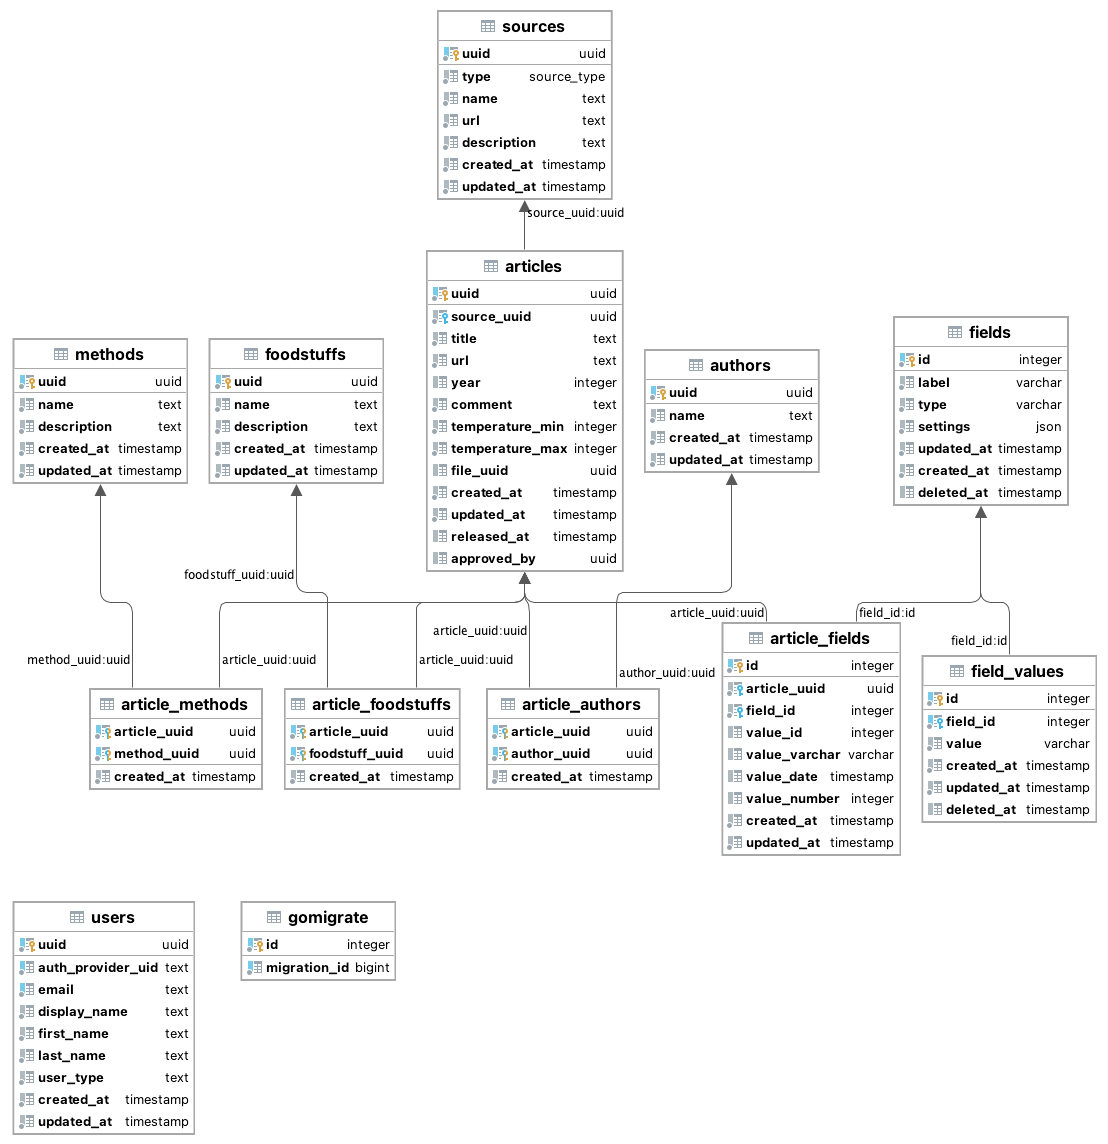
\includegraphics[width=1\textwidth]{slike/database-structure.png}
\end{center}
\caption{ Predstavitev podatkovne sheme z ER diagramom }
\label{database-diagram-er}
\end{figure}
\subsection{Pridobivanje podatkov iz podatkovne baze}
eager loading, kaj zakaj kako je implementirano .. 



\subsection{Indexi }
\subsection{Upravljanje s podatkovno shemo}
Postavitev podatkovne sheme se izvede v zbirki podatkov vsakič, ko je potreba posodobiti ali povrniti shemo baze podatkov na novo ali na starejšo različico. Ta proces imenujemo tudi migracija podatkovne sheme.

Za izvajanje migracij, v aplikaciji uporabljamo 
Migriracije se izvajajo programsko z uporabo orodja za migriranje podatkovne sheme. Ko se prikliče z določeno želeno različico sheme, orodje avtomatizira zaporedno uporabo ali razveljavitev ustreznega zaporedja sprememb sheme, dokler se ne spravi v želeno stanje.

Namen večine orodij za selitev sheme je zmanjšati vpliv sprememb sheme na vse obstoječe podatke v bazi podatkov. Kljub temu ohranitev podatkov na splošno ni zagotovljena, ker lahko spremembe sheme, kot je brisanje stolpca baze podatkov, uničijo podatke (tj. izbrišejo se vse vrednosti, shranjene v tem stolpcu za vse vrstice v tej tabeli). Namesto tega orodja pomagajo ohraniti pomen podatkov ali reorganizirati obstoječe podatke v skladu z novimi zahtevami. Ker pomena podatkov pogosto ni mogoče kodirati, konfiguracija orodij običajno zahteva ročno posredovanje.

\begin{figure}
\centering
\begin{lstlisting}[language=bash, style=mystyle]
-- Table Definition
CREATE TABLE "articles"
(
    "uuid"            uuid      NOT NULL PRIMARY KEY,
    "source_uuid"     uuid      NOT NULL REFERENCES sources (uuid) ON DELETE CASCADE,
    "title"           text      NOT NULL,
    "url"             text      NOT NULL DEFAULT '',
    "year"            int,
    "comment"         text      NOT NULL DEFAULT '',
    "temperature_min" int       NOT NULL DEFAULT 0,
    "temperature_max" int       NOT NULL DEFAULT 0,
    "file_uuid"       uuid,
    "created_at"      timestamp NOT NULL DEFAULT now(),
    "updated_at"      timestamp NOT NULL DEFAULT now()
);
\end{lstlisting}
\caption{Izsek koda, za kreiranje tabele "articles", namenjeno hranjenju podatkov o publikacijah.}
\end{figure}

\subsubsection{UUID}
Enoličen univerzalen identifikator - \verb=UUID= (angl. "Universally Unique Identifier") je standardna identifikacijska koda, ki se uporablja v postopku izdelave programske opreme. Uporablja se za ustvarjanje univerzalnih unikatnih identifikatorjev, ki omogočajo prepoznavanje in razlikovanje predmeta znotraj sistema ali istega predmeta v različnih kontekstih.

UUID je sestavljen iz 32 znakov (16 oktetov). Vsak znak je predstavljen v šestnajstiškem (heksadecimalnem) zapisu, kar pomeni, da je znak lahko število od \verb=0= do \verb=9=, ali pa črka od \verb=a= do \verb=f= (\cite{uuid-rfc}).

Glede na ime bi lahko sklepali, da je UUID unikaten glede na čas in prostor. Vendar je končno število vseh kombinacij UUID-jev $n=2^{122}$. To pomeni, da je verjetnost, da naletimo na dva enako zgenerirana identifikatorja, zelo nizka.
Pa vendar, če zgeneriramo množico UUIDjev ($r$), kjer je število generiranih identifikatorjev večje kot največje število vseh mogočih vrednosti ($r > n$), morajo v množici obstajati duplikati. Verjetnost, da se pojavijo duplikati je mogoče natančno izračunati na podlagi rojstnodnevnega paradoksa~\cite{birthday-problem-what-is}, ki ga je leta 1932 predstavil Von Mise \cite{birthday-problem-inventor}.

\begin{izrek}
\label{iz:1}
Verjetnost unikatno generiranega UUIDja
\begin{equation}
\mathtt{\frac{n!}{n^{r}(n-r)}}
\label{eq:1}
\end{equation}
\end{izrek}

\begin{dokaz}
Število načinov, da nimamo dvojnikov je $n*(n-1)*(n-2)* …(n-(r-1))$. Kar pomeni, da je lahko prvi UUID katerakoli kombinacija od $n$ možnosti, drugi je lahko katera koli kombinacija od \verb=n=, razen prvega $(n-1)$, in tako naprej $(n-2)$... Skupno število načinov za generiranje $r$ UUID-jev je torej $n^r$, saj ima vsak, od $r$ UUIDjev $n$ različnih kombinacij.
S tem je dokaz Izreka~\ref{iz:1} zaključen.
\end{dokaz}

Če nadaljujemo računanje na podlagi rosjtnodnevnega paradoksa, pridemo do rešitve, ki nam pove, da je vrjetnost resnično majhna. Da se pojavi duplikat, bi morali vsako sekundo zgenerirati miljardo vrednosti torej 85 zaporednih let. Datoteka z zgeneriranimi UUID-ji bi bila na koncu velika $45EB$ ($45kb*1000^6$) \cite{uuid-collisions}


\subsection{Podatki za testiranje}
// seederjo - fixtures

\clearpage
\section{Odlaganje datotek}
Kaksne podatke odlagamo. Kam se jih odlaga. Zakaj sem izbral tako resitev.
\subsection{Minio}
Minio je samostojna rešitev da ustvarite lastno shrambo predmetov. Je alternativa za AWS S3.

Programska oprema Minio je na voljo kot preprost binarni dokument in celo uradna dokumentacija kaže, da ga uporabljajo na tak način, namesto da uporabite upravitelja paketov. Seveda obstajajo Dockerjeve slike če jih želite uporabiti za zagon minio na vašem VPS.

Minio je bolj primeren za shranjevanje nestrukturiranih podatkov kot so fotografije, videoposnetki, dnevniške datoteke, varnostne kopije in slike vsebnikov / VM. Velikost predmeta se lahko giblje od nekaj KB do največ 5 TB.

MinIO is a High Performance Object Storage released under GNU Affero General Public License v3.0. It is API compatible with Amazon S3 cloud storage service. It can handle unstructured data such as photos, videos, log files, backups, and container images with (currently) the maximum supported object size of 5TB.[3]

\section{Varnost podatkov}

Skoraj vsaka aplikacija zahteva določeno raven sistema avtorizacije. V nekaterih primerih je dovolj, da potrdimo nabor uporabniškega imena/gesla z našo tabelo Users, vendar pogosto potrebujemo bolj natančen model dovoljenj, da nekaterim uporabnikom omogočimo dostop do določenih virov in jih omejimo pred drugimi. 
Izgradnja sistema za podporo slednjega ni nepomembna in je lahko zelo dolgotrajna. V tej vadnici se bomo naučili, kako zgraditi API za overjanje na podlagi vlog z uporabo Firebase, ki nam bo pomagal hitro zagnati in zagnati.

https://sl.portaldacalheta.pt/json-web-token-tutorial

The authentication process always runs at the start of the application, before the permission and throttling checks occur, and before any other code is allowed to proceed. Different systems may require different types of credentials to ascertain a user’s identity. The credential often takes the form of a password, which is a secret and known only to the individual and the system. Three categories in which someone may be authenticated are: something the user knows, something the user is, and something the user has.

Authentication process can be described in two distinct phases - identification and actual authentication. Identification phase provides a user identity to the security system. This identity is provided in the form of a user ID. The security system will search all the abstract objects that it knows and find the specific one of which the actual user is currently applying. Once this is done, the user has been identified. The fact that the user claims does not necessarily mean that this is true. An actual user can be mapped to other abstract user object in the system, and therefore be granted rights and permissions to the user and user must give evidence to prove his identity to the system. The process of determining claimed user identity by checking user-provided evidence is called authentication and the evidence which is provided by the user during process of authentication is called a credential.


401 Unauthorized (https://datatracker.ietf.org/doc/html/rfc7235#page-3)
Koda stanja 401 (Nepooblaščeno) pomeni, da zahteva ni bila uporabljena, ker nima veljavnih poverilnic za preverjanje pristnosti za ciljni vir. Strežnik, ki generira odgovor 401, MORA poslati naslovno polje WWW-Authenticate (razdelek 4.1), ki vsebuje vsaj en izziv, ki velja za ciljni vir.

Če je zahteva vsebovala poverilnice za preverjanje pristnosti, potem odgovor 401 kaže, da je bila avtorizacija za te poverilnice zavrnjena. Uporabniški agent LAHKO ponovi zahtevo z novim ali zamenjanim poljem glave avtorizacije (razdelek 4.2).

The "Authorization" header field allows a user agent to authenticate itself with an origin server -- usually, but not necessarily, after receiving a 401 (Unauthorized) response.  Its value consists of credentials containing the authentication information of the user agent for the realm of the resource being requested.

Authorization = credentials

If a request is authenticated and a realm specified, the same credentials are presumed to be valid for all other requests within this realm (assuming that the authentication scheme itself does not require otherwise, such as credentials that vary according to a challenge value or using synchronized clocks). (https://datatracker.ietf.org/doc/html/rfc7235#section-4.2)

\subsection{Avtorizacija na podlagi vlog}

The process of authorization is distinct from that of authentication. Whereas authentication is the process of verifying that "you are who you say you are", authorization is the process of verifying that "you are permitted to do what you are trying to do". While authorization often happens immediately after authentication (e.g., when logging into a computer system), this does not mean authorization presupposes authentication: an anonymous agent could be authorized to a limited action set.[24]


Definition: Authorization is a security mechanism to determine access levels or user/client privileges related to system resources including files, services, computer programs, data and application features. This is the process of granting or denying access to a network resource which allows the user access to various resources based on the user's identity.

Description: Most web security systems are based on a two-step process. The first step is authentication, which ensures about the user identity and the second stage is authorization, which allows the user to access the various resources based on the user's identity. Modern operating systems depend on effectively designed authorization processes to facilitate application deployment and management. Key factors contain user type, number and credentials, requiring verification and related actions and roles.

Access control in computer systems and networks relies on access policies and it is divided into two phases:

1) Policy definition phase where access is authorized.

2) Policy enforcement phase where access requests are permitted or not permitted.

Thus authorization is the function of the policy definition phase which precedes the policy enforcement phase where access requests are permitted or not permitted based on the previously defined authorizations. Access control also uses authentication to check the identity of consumers. When a consumer attempts to access a resource, the access control process investigates that the consumer has been authorized to use that resource. Authorization services are implemented by the Security Server which can control access at the level of individual files or programs.


V tem avtorizacijskem modelu je dostop dodeljen vlogam namesto določenim uporabnikom, uporabnik pa ima lahko eno ali več, odvisno od tega, kako oblikujete svoj model dovoljenja. Viri po drugi strani zahtevajo določene vloge, ki uporabniku omogočajo, da jih izvede.

Imamo 3 vrste uporabnikov. Vsi ti uporabniki se avtenticirajo z uporabo JWT zetona. 
Kaj je ta zeton? Kako so definirane razlicne pravice uporabnikov? 
Kaj je firebase, oauth, API key, JWT token, zakaj sem se odlocil za JWT token. 
Ali je smiselno razijati svojo authentikacijo ali uporabiti ze obstojeco.


Funkcije aplikacije, povezane s preverjanjem pristnosti in upravljanjem sej, se pogosto izvajajo napačno, kar napadalcem omogoča, da ogrozijo gesla, ključe ali žetone seje ali izkoriščajo druge pomanjkljivosti implementacije za začasno ali trajno prevzem identitete drugih uporabnikov.

\subsection{JWT}
https://sl.portaldacalheta.pt/json-web-token-tutorial
JWT je predstavljen kot zaporedje base64url kodirane vrednosti, ki so ločene s pikami.

Preverjanje pristnosti na osnovi žetonov nam omogoča izdelavo ločenih sistemov, ki niso vezani na določeno shemo preverjanja pristnosti. Žeton je lahko ustvarjen kjer koli in porabljen v katerem koli sistemu, ki za podpis žetona uporablja isti skrivni ključ. So pripravljeni na mobilne naprave in od nas ne zahtevajo uporabe piškotkov.

Še vedno je veliko zajeti o JWT-jih, na primer o tem, kako ravnati z varnost podrobnosti in osvežujoče žetone, ko potečejo, toda vadnica JSON Web Token bi morala prikazati osnovno uporabo in, kar je še pomembneje, prednosti uporabe JWT-jev.

JWT pomeni JSON Web Token, običajna taktika preverjanja pristnosti, ki se uporablja v sodobnih spletnih aplikacijah.

\subsection{HTTPS}
Definition: HTTPS stands for Hypertext Transfer Protocol Secure. It is the protocol where encrypted HTTP data is transferred over a secure connection. By using secure connection such as Transport Layer Security or Secure Sockets Layer, the privacy and integrity of data are maintained and authentication of websites is also validated.

Description: HTTPS ensures data security over the network - mainly public networks like Wi-Fi. HTTP is not encrypted and is vulnerable to attackers who are eavesdropping and can gain access to website database and sensitive information. By virtue, HTTPS encryption is done bi-directionally, which means that the data is encrypted at both the client and server sides. Only the client can decode the information that comes from the server. So, HTTPS does encryption of data between a client and a server, which protects against eavesdropping, forging of information and tampering of data. But how do you ensure if you are seeing an HTTPS-enabled web page? Just check the address bar that carries the site name against different background colours with a lock icon at the left corner. However, this design can be different for different browsers. For example, consider going to a bank website, say hdfcbank.com. A non-secured HTTP will open up. But when we go to the login page, we can see an HTTPS in the address bar with some specific design. Implementation: HTTPS is mainly used by those websites which deal with monetary transactions or transfer user's personal data which could be highly sensitive. Banking websites are common examples. In layman's terms, HTTPS ensures that users watch websites that they want to watch. Data exchanged between the user and the website is not read, stolen or tampered with by a third party. But it can't encrypt everything - it has some limitations too. For example, HTTPS can't encrypt host addresses and port numbers.

\subsection{Secure Sockets Layer - SSL}
Definition: Secure Sockets Layer (SSL) is a protocol developed by Netscape for establishing an encrypted link between a web server and a browser. SSL is an industry standard which transmits private data securely over the Internet by encrypting it. It is used by many websites to protect the online transactions of their customers.

Description: SSL functions around a cryptographic system which uses three keys to set up the SSL connection: public, private, and session keys. Anything encrypted by using the public key can only be decrypted with the private key, and vice versa. SSL Certificate will contain the company name, address, city, state, country, domain name, expiration date of the Certificate and details of the Certification Authority responsible for issuing the Certificate. When a browser connects to a secure site, it retrieves the website's SSL Certificate that authenticates that it has not expired, and that it has been issued by a Certification Authority the browser trusts. If it fails on any of these checks, the browser displays a warning message to the end user, letting them know that the site is not secured by SSL. Many websites use the protocol to collect confidential user information, including credit card numbers. Most web browsers support SSL. SSL connection URL starts with 'https:' instead of 'http:'. The complexities of the SSL protocol remain invisible to the customers. The lock icon in the lower right-hand corner in the browser displays the SSL Certificate and when the icon is clicked, it displays the whole description about the Certificate.

\subsection{SQL injection}
Definition: SQL injection is an application layer attack technique used by hackers to steal data from organizations by targeting web-based applications.

Description: SQL injection is one of the methods by which hackers attack the underlying data storage of a web application by taking advantage of improper coding styles or insufficient database privileges assigned to the application user who accesses this database. SQL injection arises because user input fields - if not checked correctly at the application - allow SQL statements to pass through and directly question the database, allowing attackers to tamper with or even delete existing data, spoof identity, change administrative rights and in some cases void transactions and change balances. For example, consider a generic login page wherein users can enter their usernames and passwords where they can view their personal details or modify them. Once the user submits the details, an SQL query is generated from these details and sent to the database for verification. If found legitimate, the user is allowed access. Now through SQL injection, the attacker may insert some specifically-crafted SQL commands to bypass the login form and see what lies behind it. Inputs that are not properly sanitized (i.e. made invulnerable) will make this possible and be sent directly with the SQL query to the database, following which the attacker will gain access to the database

\subsection{Middleware}

\subsection{Firebase}
https://www.toptal.com/firebase/role-based-firebase-authentication
Na kratko, preverjanje pristnosti Firebase je razširljiv sistem za preverjanje pristnosti, ki temelji na žetonih, in zagotavlja izključene integracije z najpogostejšimi ponudniki, kot so Google, Facebook in Twitter, in ostali.

Omogoča nam uporabo zahtevkov po meri, ki jih bomo izkoristili za izgradnjo prilagodljivega API-ja, ki temelji na vlogah.

V zahtevke lahko nastavimo katero koli vrednost JSON (npr. { "vloga": 'administrator' } ali { "vloga": 'urednik' }).

Ko so nastavljeni, bodo zahtevki po meri vključeni v žeton, ki ga ustvari Firebase, in lahko preberemo vrednost za nadzor dostopa.

Prihaja tudi z zelo velikodušno brezplačno kvoto, ki je za potrebo projekta vec kot dovolj.

Account creation and deletion limits
Operation	Limit
New account creation	100 accounts/IP address/hour
Account deletion	10 accounts/second
Registered user accounts	unlimited

https://firebase.google.com/docs/auth/limits



\section{Validiranje podatkov}

Kako se podatki validirajo. Kako se dinamicni podatki predstavijo v API-ju..
Kaj se zgodi ze se kaksen podatak izgubi/izbrise? Kako se to resuje na razlicnih podatkovnih bazah. Odvisno od zahtev...


\section{Vue.js}
\label{vue-js-section}
Vue (prebran $/vju/$, kot angl. view) je odprtokodno, progresivno \verb=JavaScript= ogrodje (angl. framework), namenjeno izdelavi uporabniških vmesnikov in enostranskih aplikacij.

Vue.js ima postopoma prilagodljivo arhitekturo, ki se osredotoča na deklarativno upodabljanje in sestavo komponent. Jedrna knjižnica je osredotočena samo na vizualni sloj. Napredne funkcije, potrebne za zapletene aplikacije, kot so usmerjanje, upravljanje stanja in orodja za gradnjo, so na voljo prek uradno vzdrževanih podpornih knjižnic in paketov \cite{vue-js-what-is}.


\section{Tezave ki sem jih imel}
https://www.toptal.com/go/golang-oop-tutorial

Tukaj opisem na kaksne tezave sem naletel med razvojem aplikacije.

\chapter{Predstavitev Aplikacije}
V prejšnjem poglavju smo spoznali posamezne tehnologije in orodja, ki smo jih uporabili za izvedbo naše aplikacije. V naslednjem sklopu pa bomo spoznali kako smo omenjene tehnologije in orodja uporabili. 

Aplikacija je sestavljena iz zalednega in čelnega dela. Zaledni del, je sestavljen iz večih komponent, in sledi arhitekturni postavitvi mikrostoritev. Čelni del pa je enostavna aplikacija, napisana v programskem ogrodju \verb=vue.js=. To je del aplikacije, ki je prikazan uporabniku, zato je pomembno, da je na videz enostaven in pregleden, hkrati pa tudi hiter in funkcionalen. 

\section{Postavitev projekta v lokalnem okolju}

Namen dobrega razvojnega okolja je, da ima uporabnik (programer), možnost rekonstruiranje celotnega razvojnega okolja z čim manj vloženega truda. To mu zagotavlja, da projekt povrne v stanje, ki ga imajo vsi ostali programerji, in s tem izniči velik delež samostojne napake, ki se lahko zgodi pri programiranju programske opreme. Velikokrat se lahko zgodi da je težava v infrastruktuiri, zaradi napačne postavitve samega projekta. Tej težavi smo se hoteli izogniti z pravilno postavitvijo projekta.

Za naš projekt, smo se odločili za uporabno vsebovalnikov (angl. containers). Sama implementacija je narejena z uporabno orodja \verb=Docker=. Izvedba je nostavna in je definirana z konfiguracijskimi datotekami. Za zagon projekta je potrebno imeti prednameščeni orodji \verb=Docker= in \verb=Git=.

Z uporabo orodja \verb=Git=, je potrebno prenesti celoten projekt na razvijalčev računalnik. Razvijalec mora imeti dostop do repozitorija, ki je na voljo na platformi \verb=GitHub=. Ko ima razvijalec vse potrebne dostope in pravice, mu je omogočen prenos vseh datotek na njegov računalnik. 
To stori z ukazom Ukaz \ref{lst:git-clone}.

\begin{lstlisting}[language=bash,style=mystyle,caption={Uporaba orodja Git, za prenos projekta},label=lst:git-clone]
$ git clone git@github.com:marolt/diploma.git
\end{lstlisting}

\subsection{Postavitev zalednega dela aplikacije}
Zagon aplikacje je odvisen kar od nekaj komponent. Za medsebojno delovanje in odvisnost vsebnikov poskrbi orodje \verb=docker-compose=. Docker Compose je ogrodje razvito okrog Docker sistema, ki nam omogoča enostavno orkestracijo vsebovalnikov. Z definiranjem konfiguracijske datoteke \verb=docker-compose.yml= (Koda \ref{lst:dco-snipet}), smo nastavili povezave med posameznimi storitvami, kakšna vrsta omrežja naj bo uporabljena, spremeljivke okolja, katero sliko vsebovalnika naj posamezna storitev uporabi, katera vrata naj odpre na gostitelja, in se ostale stvari, ki so potrebne za postavitev celotne arhitekture.

Za vsako storitev je definiran vsebovalnik, ki ima definirano katero sliko naj uporabi. Za zaganjanje programske kode v go programskem jeziku, medtem ko smo aplikacijo razvijali, smo zraven osnovne slike pripeli še dodatno orodje za osveževanje kode \ref{lst:dcf-snipet}.

\begin{lstlisting}[style=mystyle,caption={Dockerfile datoteka za razvijanje Go programske opreme},label=lst:dcf-snipet]
FROM golang:1.17
RUN go get github.com/cespare/reflex
COPY reflex.conf /
COPY run.sh /
ENTRYPOINT ["reflex", "-c", "/reflex.conf"]
\end{lstlisting}


Uporabili smo osnovno sliko $\verb=golang:1.17=$, ki je uradna slika iz strani razvijalcev programskega jezika Go. Naslednji ukaz $\verb=RUN=$ zažene ukaz za namestitev orodja $\verb=reflex=$, ki omogoča sprotno osveževanje kode med samim razvojem v programskem jeziku Go. Ukaz $\verb=COPY=$ prekopira datoteko $\verb=reflex.conf=$ in $\verb=run.sh=$ iz gostiteljevega datotečnega sistema. Zadnji ukaz v datoteki, $\verb=ENTRYPOINT=$ pa zažene ukaz $\verb=reflex=$ z dodatnimi parametri, ki definirajo konfiguracijko datoteko. Ta ukaz se bo vedno zagnal ob vsakem zagonu vsebovalnika.

\begin{lstlisting}[style=mystyle,caption={Izsek konfiguracijske datoteke docker-compose.yml},label=lst:dco-snipet]
version: '3'
services:
  db:
    image: postgres:9.6.23
    env_file:
      - docker.env
    ports:
      - "5433:5432"
    volumes:
      - postgresql-data:/var/lib/postgresql/data/
  app:
    build:
      context: docker/app
    volumes:
      - .:/src
    working_dir: /src/articles
    ports:
      - "3000:80"
    env_file:
      - .env
    depends_on:
      - minio
      - db
  minio:
    image: minio/minio
    volumes:
      - minio-volume:/export
    ports:
      - "9000:9000"
    command: server /export
volumes:
...
\end{lstlisting}
V izseku kode (\ref{lst:dco-snipet}) lahko vidimo, kako so posamezni vsebovalniki definirani v datoteki docker-compose.yml. Razvidna je tudi njihova medsebojna odvisnost, kot naprimer za delovanje vsebovalnika $app$ je potrebno, da sta dosegljiva tudi ostala dva vsebovalnika ($db$ in $minio$).

Da je delo na projektu še bolj enostavno smo ukaze ovili z orodjem \verb=Makefile=. To orodje nam omogoča, definiranje opravil, ki zaženejo sklop ukazov (ali skripto). 

\begin{lstlisting}[language=bash,style=mystyle]
$ make start
\end{lstlisting}

Zgornji ukaz poskrbi za postavitev našega projekta v okolju za razvijanje. V ozadju se izvede niz ukazov, ki zagotovijo, da so vse storitve na voljo. To lahko preverimo z ukazon $\verb=docker-compose ps=$ (Koda \ref{lst:running-containers}), kjer se izpiše aktivno stanje zagnanih vsebovalnikov. Iz izpisanega, lahko razberemo, da se ob postavitvi projekta zažene devet vsebovalnikov.  

\begin{lstlisting}[language=bash,style=mystyle,caption={Prikaz zagnanih vsebovalnikov},label=lst:running-containers]
$ docker-compose ps

Name           Command                State  Ports
------------------------------------------------------------
d_web_1        /run.sh.                 Up   :80->80/tcp
d_app_1        reflex -c /reflex.conf   Up   :3002->80/tcp
d_users_1      reflex -c /reflex.conf   Up   :3001->80/tcp 
d_firestore_1  dockerize -template=/... Up   :9099->9099/tcp             
                                             8787/tcp
d_minio_1      /usr/bin/docker-entry... Up   9000/tcp     
d_memcached_1  docker-entrypoint.sh ... Up   11211/tcp     
d_postgres_1   docker-entrypoint.sh ... Up   :5433->5432/tcp       
d_trace_1      /go/bin/all-in-one-linux Up   14250/tcp 
                                            :14268->14268/tcp
                                            :16686->16686/tcp
                                            5775/udp,5778/tcp 
                                            6831/udp,6832/udp   
d_teus_1       /bin/prometheus --con... Up  9090/tcp     
\end{lstlisting}

Za razvojno okolje, nekaterih storitev ni smiselno izolirati na nivoju infrastrukture. V našem primeru si naše storitve delijo skupni vsebovalnik za podatkovno bazo, in s tem prihranimo na hitrosti lokalnega razvoja. Razvoj aplikacije je v našem primeru enostavnejši in preglednejši, vendar moramo biti med razvojem pazljivi, da ohranimo medsebojno neodvisnost samih storitev. 

Za lažjo predstavitev, nam je na voljo diagram celotne arhitekure prikazan na sliki \ref{final-arch}

\begin{figure}[h]
\begin{center}
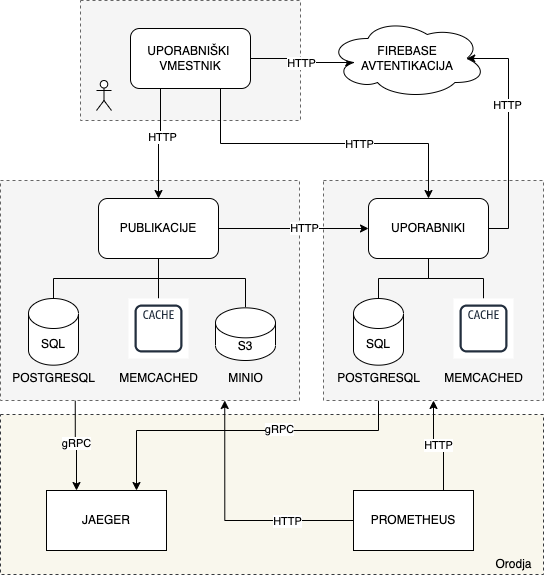
\includegraphics[width=0.75\textwidth]{slike/arch-done.png}
\end{center}
\caption{ Arhitektura projekta predstavljena z diagramom }
\label{final-arch}
\end{figure}

\subsection{Postavitev čelnega dela aplikacije}
Čelni sistem uporablja $\verb=javaScript=$ ogrodje \verb=vue.js=. Ogrodje je odvisno od \verb=node.js= programskih datotek, zatorej moramo v sliko vsebovalnika namestiti potrebne stvari za delovanje tega ogrodja. 

V namšem primeru (Koda: \ref{lst:dcf-node}) uporabimo pred definirano sliko \\ \texttt{node:17.3.0-alpine3.14}, ki že ima nameščena orodja kot so \texttt{node.js} in upravljec paketkov \texttt{npm}. Ker je vmestnik uporabljen v razvojnem okolju, definiramo vrednost \texttt{NODE\_ENV} na \texttt{development}. Skripta \texttt{run.sh} je skopirana v sliko z dodatnimi pravicami, za zagon. Na koncu se skipto sproži v izvajanje.

\begin{lstlisting}[,style=mystyle,caption={Dockerfile datoteka za razvijanje Vue aplikacije},label=lst:dcf-node]
FROM node:17.3.0-alpine3.14

ENV NODE_ENV development

ADD start.sh /
RUN chmod +x /start.sh

CMD ["/run.sh"]
\end{lstlisting}

V datoteki $start.sh$ (\ref{lst:dcf-run}) so navedeni ukazi, ki se zgodijo ob vsakem zagonu vsebovalnika. Komanda \texttt{npm install} namesti vse potrebne knjižnjice, ki jih v aplikaciji uporabljamo. Komanda \texttt{npm serve} pa zažene spletni strežnik, ki streže vsebino aplikacije iz trenutnega direktorija.

\begin{lstlisting}[language=bash,style=mystyle,caption={Ukazna datoteka, ki nasneme potrebne knjižnice in streže aplikacijo},label=lst:dcf-run]
set -e

npm install
npm serve
\end{lstlisting}

Pomembno je tudi poudariti, da je aplikacija enostranska (angl. single-page), kar pomeni, da deluje znotraj brskalnika in ne potrebuje ponovnega nalaganja strani med svojim delovanjem. Je le ena sama stran, ki jo obiščemo in na kateri se nato naloži vso ostalo vsebino s pomočjo JavaScripta.

Kot je razvidno iz prikaza zagnanih vsebovalnikov (Koda: \ref{lst:running-containers}), ima čelni del odprta vrata 80, kar pomeni, da je stran dostopna na lokalnem spletnem naslovu \url{http://localhost:80/}. 


\section{Čelni del aplikacije}
V tem delu bomo spoznali kaj je čelni del naše aplikacije in s katerimi tehnologijami je sestavljen. Pri razvoju čelnega sistema je potrebno biti pozoren na kar nekaj stvari, kot je naprimer zasnova na videz lepega, vendar uporabnega grafičnega vmestnika. Preko tega vizialnega vmestnika uporabnik varno komunicira z našim zalednim sistemom. Med samo uporabo in komunikacijo ne smemo pozabiti na ustrezno prikazovanje napak uporabniku, da sam uporabnik ve kdaj je do napake prišlo in kako jo odpraviti.

Čelni del aplikacije uporablja ogrodje \verb=Vue.js= (\ref{vue-js-section}), ki je zelo enostavno \verb=JavaScript= ogrodje z številnimi orodji in knjižnicami, s katerimi si poenostavimo in pohitrimo razvoj. Knjižnice, ki jih aplikacija potrebuje, so navedene v datoteki \verb=packgage.js= (\ref{lst:pkg-snippet}). V omenjeni datoteki so navedeni tudi ukazi, s katerimi prožimo določene akcije, kot so gradnja statičnih paketov, postavitev spletnega strežnika za streženje datotek in gradnja css datotek z pomočjo knjižnice \verb=tailwind=. 

\begin{figure}
\centering
\begin{lstlisting}[language=php, style=mystyle,caption={Dockerfile datoteka za razvijanje Vue aplikacije},label=lst:pkg-snippet]
{
  "name": "diploma",
  "version": "1.0.0",
  "private": true,
  "scripts": {
    "serve": "vue-cli-service serve",
    "build": "vue-cli-service build",
    "lint": "vue-cli-service lint",
    "build:tailwind": "npx tailwindcss ...",
    "install:clean": "rm -rf node_modules/ ..."
  },
  "dependencies": {
    "@fortawesome/fontawesome-free": "^5.15.4",
    "@tailwindcss/forms": "^0.3.4",
    "@vueform/multiselect": "^2.2.1",
    "@vueform/slider": "^2.0.8",
    "core-js": "^3.19.1",
    "firebase": "^9.3.0",
    "jsonwebtoken": "^8.5.1",
    "litepie-datepicker": "^1.0.14",
    "lodash": "^4.17.21",
    "moment-timezone": "^0.5.34",
    "register-service-worker": "^1.7.1",
    "superagent": "^6.1.0",
    "v-tooltip": "^4.0.0-beta.2",
    "vue": "^3.2.21",
    "vue-router": "^4.0.0-0",
    "vue-toast-notification": "^2.0.1"
  },
  "devDependencies": {
     ...
    "sass": "^1.32.5",
    "sass-loader": "^10.1.1",
    "tailwindcss": "^2.2.19"
  }
}

\end{lstlisting}
\caption{Primer validacijske funkcije za uporabnisko ime, z uporabo regularnega izraza}
\end{figure}


\section{Opis posamzenih strani}

Aplikacija je sestavljena iz 


\section{Pozdravna stran}
Ob obisku spletnega mesta \url{http://localhost/} se odpre \sn{Pozdravna stran} (Slika \ref{landing-page}). Stran je namenjena vsem uporabnikom, da se seznanijo z aplikacijo. Vsebuje povezave na zunanje vire, kjer lahko uporabnik pridobi koristne informacije o živilih. 

S klikom na gumb \sn{VSTOPI V APLIKACIJO}, je uporabnik usmerjen v aplikacijo. Če, kot uporabnik ni prijavljen, se mu odpre stran za prijavo (\ref{sign-in-page}). V primeru, da je že prijavljen, se pravi, ima tekočo sejo, pa se mu odpre domača stran znotraj aplikacije, kjer lahko uporabnik prebera in izvaja filtre nad vnešenimi publicitetami (\ref{filters-page}).

\begin{figure}[h]
\begin{center}
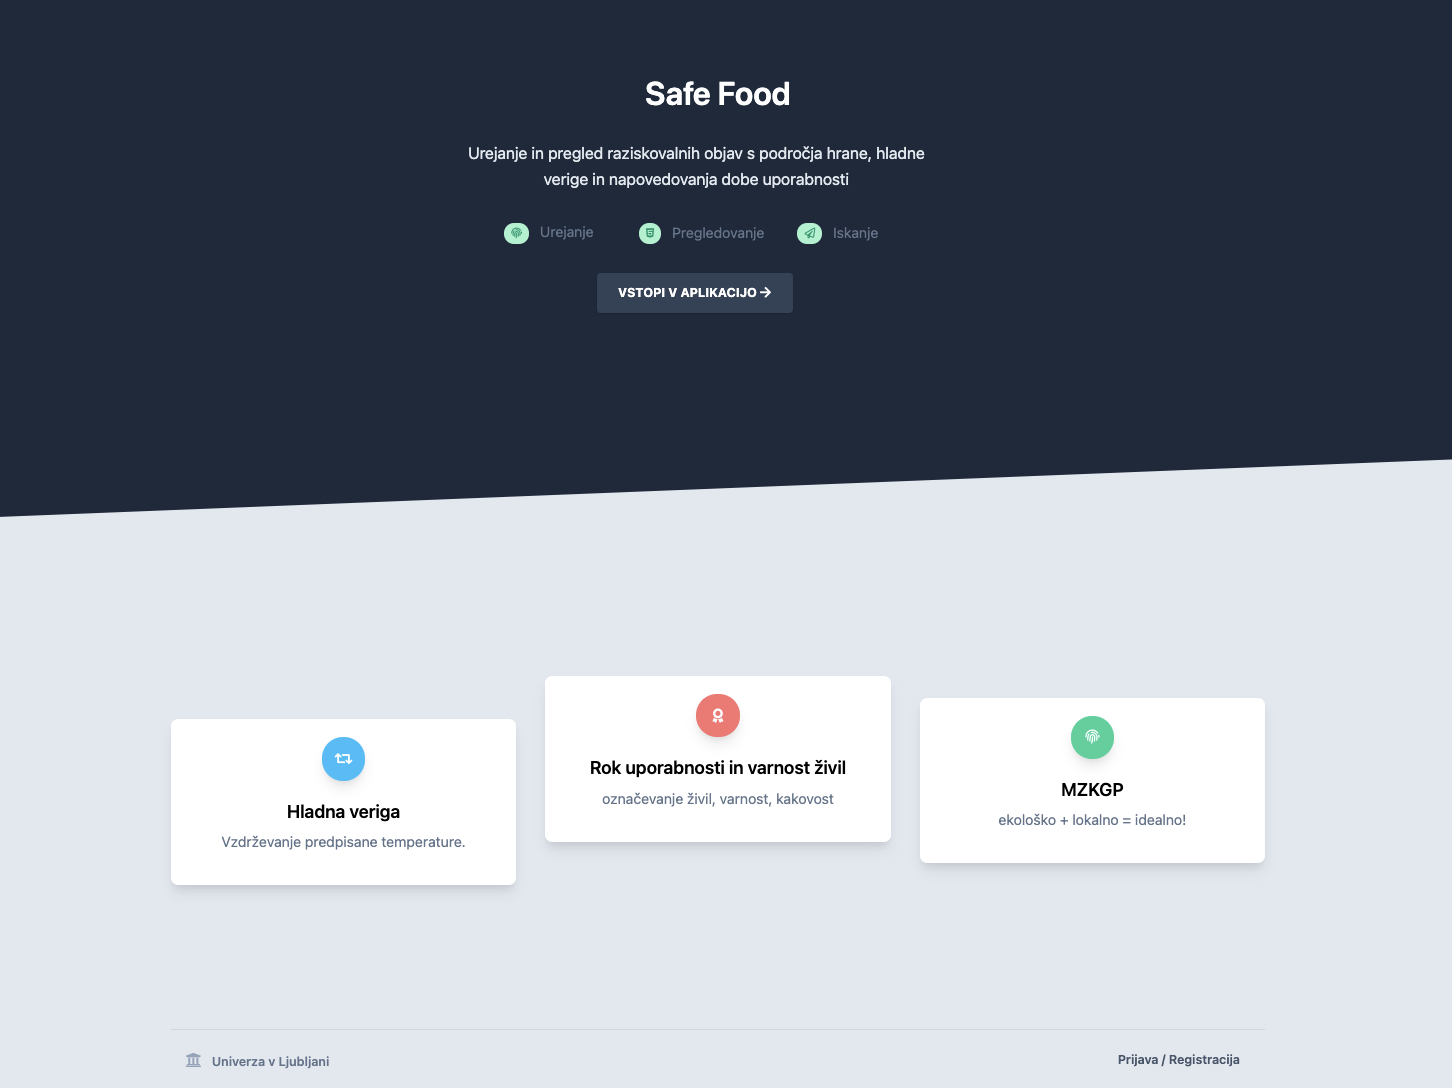
\includegraphics[width=1\textwidth]{slike/landing-page.png}
\end{center}
\caption{ Pozdravna stran }
\label{landing-page}
\end{figure}

\newpage
\section{Stran za registracijo}
\label{registration-page}
Za uporabo aplikacije je potrebna registracija uporabnika. Uporabnikom, ki se niso registrirani v aplikacijo, je dana možnost, da si kreirajo račun (Slika \ref{signup-form}).

\begin{figure}[h]
\begin{center}
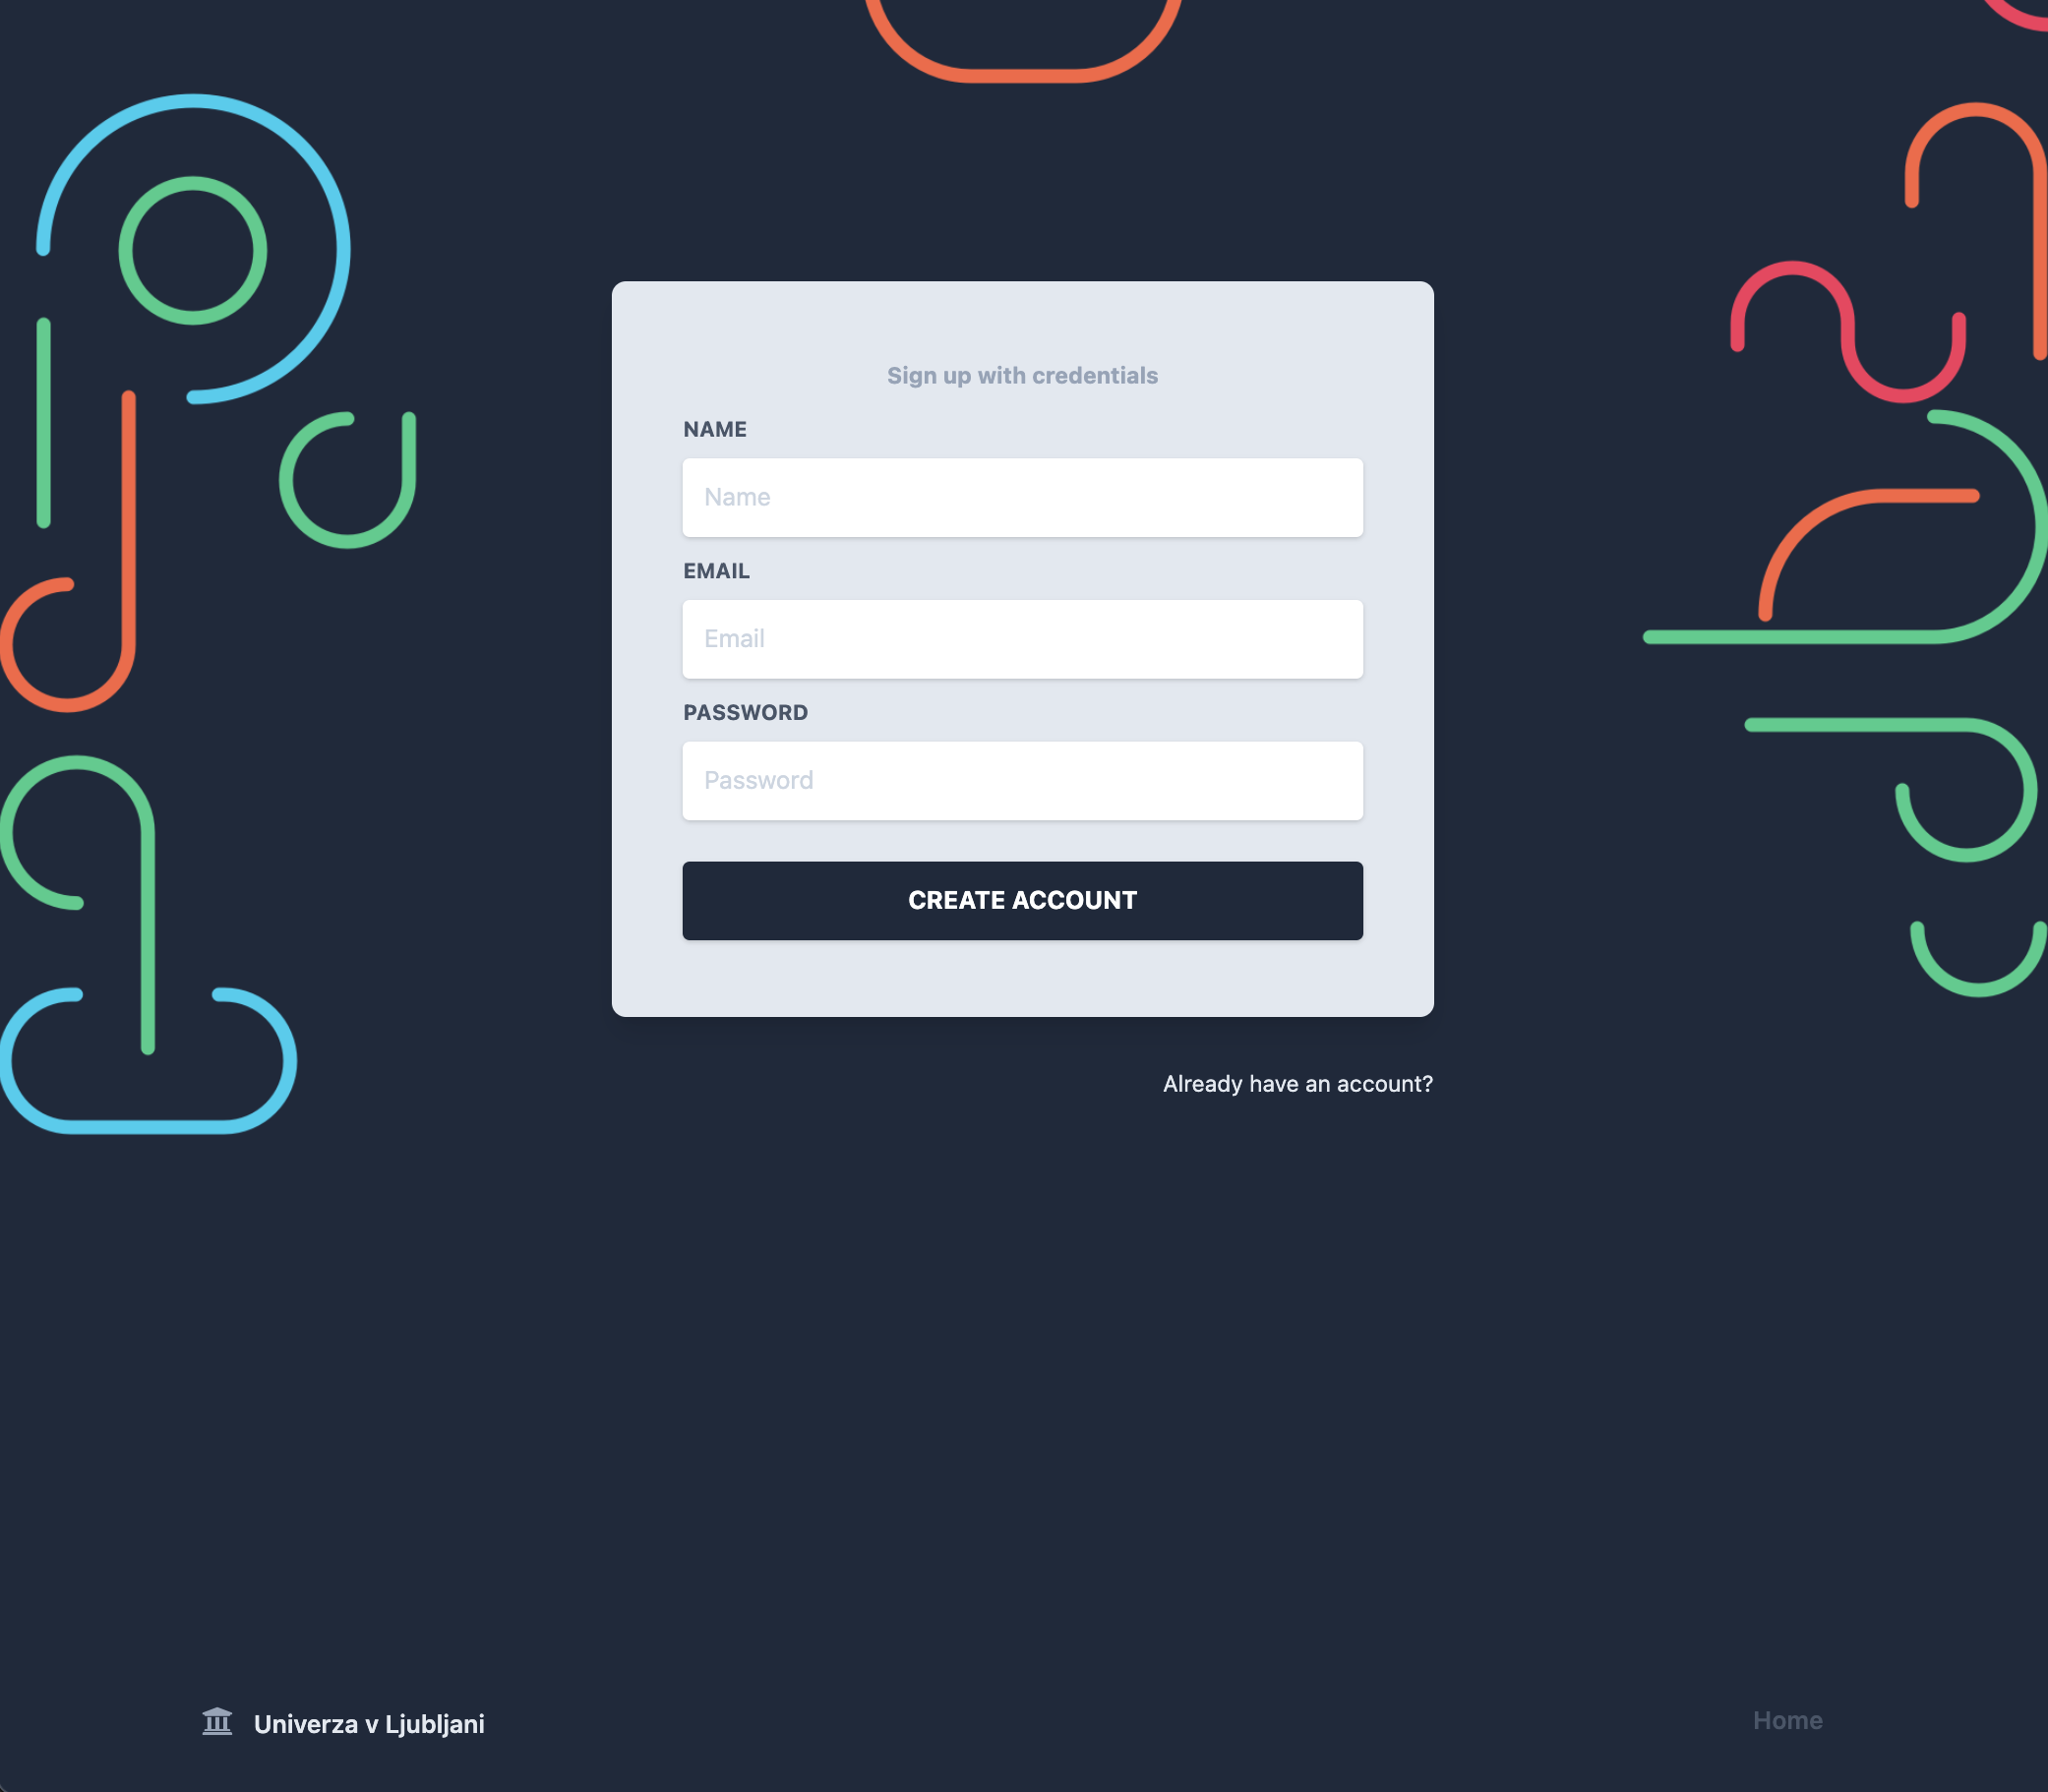
\includegraphics[width=1\textwidth]{slike/signup.png}
\end{center}
\caption{ Registracijska forma }
\label{signup-form}
\end{figure}

Uporabniško ime mora ustrezati definiranemu formatu, ki je določen kot regularni izraz in mora vsebovati vsaj tri znake (\ref{lst:validation}). V primeru, da uporabnik vnese napačno uporabniško ime ali geslo, se na vrhu vnosnih polj izpiše ustrezno opozorilo o napaki. Validacija se izvaja na zalednem iz čelnem delu.

\begin{figure}
\centering
\begin{lstlisting}[language=java, style=mystyle,caption={Primer validacijske funkcije za preverjanje uporabniškega imena z uporabo regularnega izraza},label=lst:validation]
function validateUsername(uname) {
  /*
    Uporabnisko ime, ne sme biti krajse od treh znakov
  */
  if(uname.length < 3) {
    return false;
  }

  /* 
    Vsebuje lahko le: 
    - male crke (a-z) 
    - stevilke (0-9)
    - pike (.)
    - podcrtaje (_)
  */
  const match = /^[a-z0-9_\.]+$/.exec(uname);
  
  // veljavno ali ne
  return Boolean(rezultat);
}
\end{lstlisting}
\end{figure}


Ob registraciji, uporabnik na vnešen elektronski naslov prejme novo sporočilo za potrditev uporabniskega racuna. To sporočilo je namenjeno zagotavljanju verodostonjosti uporabnika, s potrditvenim sporočilom. V primeru, da uporabnik ne potrdi njegovega poštnega predala v roku enega dneva, mu je dostop do aplikacije onemogocen, vse dokler uporabik ne potrdi računa.

Nepotrjen uporabnik nima dostopa do dela aplikacije, kjer so prikazane publikacije. Pokaže se mu le stran z navodili, kako potrditi poštni naslov. V primeru, da uporabnik ni prejel potrditevega sporočila, lahko klikne na gumb, in sproži ponovno pošiljanje potrditevega sporocil. Sporočilo bo bilo ponovno zgenerirano le v primeru, da je minila vsaj ena ura od zadnjega poizkusa pošiljanja tega sporočila.

Nenazadnje pa lahko tudi kontaktira sluzbo za pomoc uporabnikom. V tem primeru se uporabniku odpre prevzeti postni odjemalec, kamor napise elektronsko sporocilo in ga pošlje na dan elektronski naslov.

Vsak uporabnik je ob registraciji le navaden uporabnik. Vlogo uporabnika lahko spremeni le administrator, v administracijskem delu aplikacije. O tem bomo govorili v sekciji "Administracija uporabnikov" (\ref{administracija-uporabnikov}).

V elektronskem sporočilu, ki ga uporabnik prejme na svoj poštni naslov, je navedena povezava do naše aplikacije. Generirana povezava vsebuje parameter \verb="method"=, ki nam pove, katera akcija se mora izvesti, ko uporabnik odpre stran. Vue komponenta, prebere url parameter, in glede na prebran parameter sproži ustrezno akcijo na autentikacijski servis. Implementirane imamo akcijo za ponastavitev gesla in pa akcijo za potrditev poštnega naslova (\ref{auth-methods}).

\begin{figure}[h]
\begin{center}
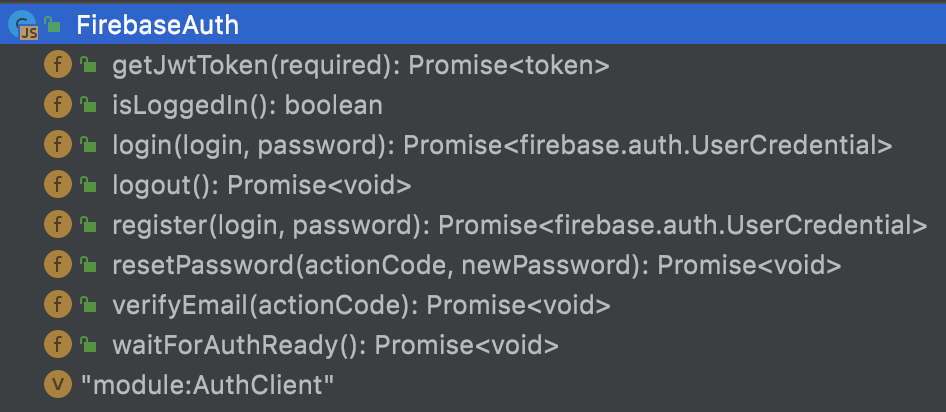
\includegraphics[width=1\textwidth]{slike/firebase_auth.png}
\end{center}
\caption{ Prikaz metod za implementacijo avtentikacijskega servisa }
\label{auth-methods}
\end{figure}

V primeru, da je uporabniški račun uspešno potrjen, je uporabnik preusmerjen na zaćetno stran aplikacije, kjer lahko izvaja iskanje nad vnešenimi publicitetami. Zgodi pa se lahko tudi, da postni naslov ni uspešno potrjen. Do slednjega primera pa lahko pride v naslednjih primerih:
\begin{myitemize}
  \item potrditvena koda je potekla
  \item neveljavna potrditvena koda
  \item izbrisan uporabniški račun
  \item onemogočen uporabniški račun
\end{myitemize}

\begin{figure}
\centering
\begin{lstlisting}[language=bash, style=mystyle]
  mounted() {
    // http://localhost:8080/auth/firebase?mode=resetPassword&oobCode={code}
    this.mode = queryParams.mode;
    this.oobCode = queryParams.oobCode;

    if (this.mode === "verifyEmail") {
      verifyAccount(this.oobCode).then(() => {
          this.$toast.success("Email verified");
          this.$router.push("home");
        }, (error) => {
          switch (error.code) {
            case 'auth/expired-action-code':
              this.$toast.error('Code expired!')
              break;
            case 'auth/invalid-action-code':
              this.$toast.error('The code is not valid.')
              break
            case 'auth/user-disabled':
              this.$toast.error('Account is disabled, please contact us at support@example.com')
              break
            case 'auth/user-not-found':
              this.$toast.error('Your account has been removed')
              break
            default:
              this.$toast.error('Email verification failed!')
          }
        });
    }
  }
\end{lstlisting}
\caption{Primer kode, za verificiranje uporabnika}
\end{figure}



\section{Prijavna stran}
\label{sign-in-page}
Uporabnik z obstoječim uporabniškim računom se lahko prijavi z uporabniškim imenom in geslom. V primeru, da je geslo pozabil, lahko s klikom na \sn{Pozabljeno geslo} nadaljuje na stran, kjer se mu odpre stran, za ponastavitev gesla (\ref{forgotten-form}). Implementirali smo tudi varnostni mehanizem, ki preprečuje uporabniku ugibati gesla. V primeru, da je uporabnik poizkusil že več kot dvajeset kombinacij gesla, se mu prijavo upočasni na deset na minuto. 
\begin{figure}
\begin{center}
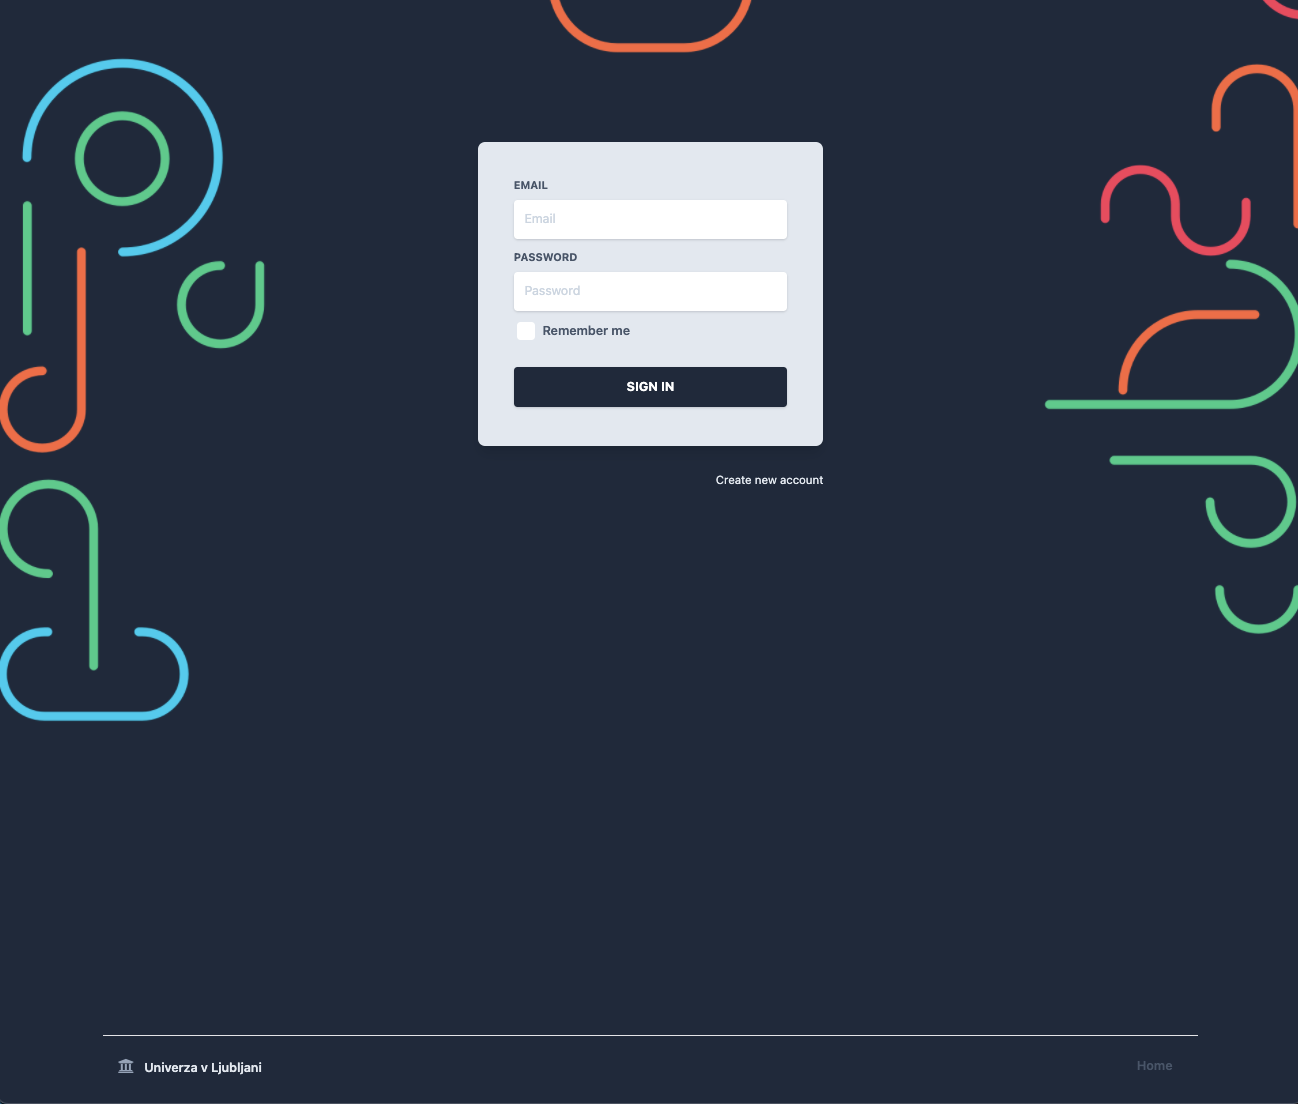
\includegraphics[width=1\textwidth]{slike/login-page.png}
\end{center}
\caption{ Prijavna stran }
\label{login-form}
\end{figure}

\section{Pozabljeno geslo}
\label{forgotten-form}
Uporabnik ima možnost obnovitve pozabljenega gesla. S klikom na gumb, se mu odpre pojavno okno, kamor vnese poštni naslov, s katerim je uporabnik identificiran v aplikacijo. Na vnešen poštni naslov, se pošlje sporočilo, ki zajema unikatno zgeneriran URL, preko katerega ima uporabnik možnost določitve novega gesla za njegov račun. 

Ob uspešni nastavitvi gesla, je uporabik preusmerjen na prijavno stran, kjer se mora prijaviti z geslom, ki ga je pravkar nastavil.

\begin{figure}[h]
\begin{center}
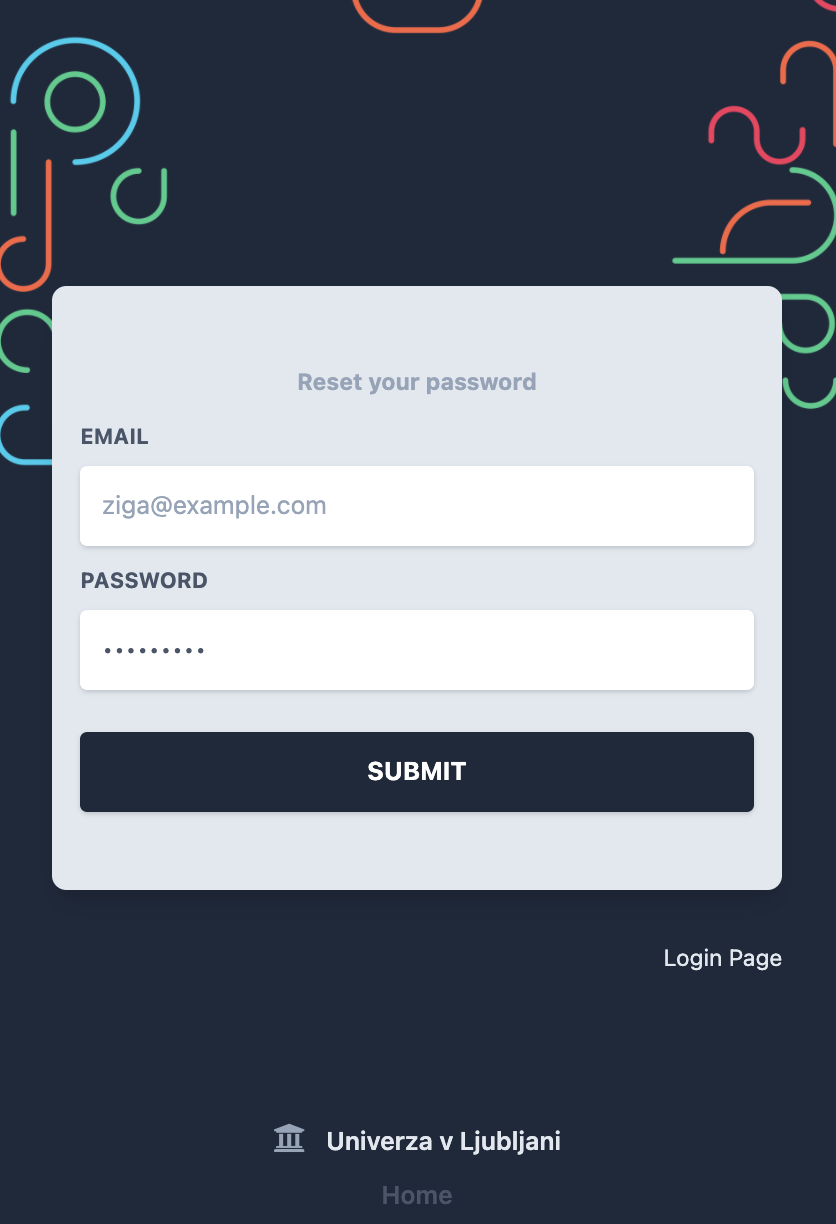
\includegraphics[width=0.5\textwidth]{slike/reset_password.png}
\end{center}
\caption{ Vnos novega gesla }
\label{password-reset-form}
\end{figure}

\section{Urejanje uporabnikov}
\label{administracija-uporabnikov}
Administrator ima dostop do strani za urejanje uporabnikov. 

\section{Razvoj dinamičnega dodajanja podatkov}
Za potrebo aplikacije smo razvili popolnoma dinamičen način za dodajanje posameznih podatkov. Uporabnik s uporabniškimi pravicami \sn{urednik}, ali \sn{administrator}, ima možnost definiranja novih parametrov za publicitacijo. Nove parametre lahko definira na strani ----FIELDS----. 

\section{Vnos podatkov}

\subsection{Transakcije}

Transakcije niso dovolj, razen če sistem prestane test ACID. ACID pomeni atomičnost, doslednost, izolacijo in trajnost. To so tesno povezana merila, ki jih mora izpolnjevati dobro veden sistem obdelave transakcij:
Atomičnost
Transakcija mora delovati kot ena sama nedeljiva enota dela, tako da se celotna transakcija uporabi ali povrne nazaj. Ko so transakcije atomične, ni delno dokončane transakcije: je vse ali nič.
  6 | 1. poglavje: Arhitektura in zgodovina MySQL
Doslednost
Baza podatkov naj se vedno premika iz enega skladnega stanja v drugo. V našem primeru doslednost zagotavlja, da zrušitev med vrsticami 3 in 4 ne povzroči, da 200 USD izgine s tekočega računa. Ker transakcija ni nikoli potrjena, se nobena od sprememb transakcije nikoli ne odraža v bazi podatkov.
Izolacija
Rezultati transakcije so običajno nevidni drugim transakcijam, dokler transakcija ni zaključena. To zagotavlja, da če se povzetek bančnega računa izvaja po vrstici 3, vendar pred vrstico 4 v našem primeru, bo še vedno videl 200 USD na tekočem računu. Ko bomo razpravljali o stopnjah izolacije, boste razumeli, zakaj smo rekli, da je običajno neviden.
Vzdržljivost
Ko so transakcije sprejete, so spremembe trajne. To pomeni, da je treba spremembe zabeležiti tako, da se podatki ne izgubijo ob zrušitvi sistema. Vzdržljivost pa je nekoliko mehak koncept, ker je dejansko veliko stopenj. Nekatere strategije trajnosti zagotavljajo močnejšo varnostno garancijo kot druge in nič nikoli ni 100-odstotno trajno (če bi bila sama baza podatkov resnično trpežna, kako bi potem varnostne kopije lahko povečale vzdržljivost?). Kaj v resnici pomeni trajnost v MySQL, bomo razpravljali v naslednjih poglavjih.


\subsection{Tipi podatkov}
Vsak podatek mora imeti definiran tip. Glede na tip podatka se razlicno vnasa in prikazuje podatek. 

\subsubsection{Vnosno Polje}
Predstavlja podatek ki ga je potrebno vnesti vsakic znova in nima definirane nobene v naprej dolocene vrednosti. Vnosno polje je lahko predstavljeno kot stevilcna vrednost, ali pa kot tekstovno polje. 
Imamo možnost vnosa mnogih vrednosti za ta podatek, tako da definiramo podatek kot ponavljajoc podatek ("repeatable"). To nam pride prav v primeru, kot je, ce hocemo dodati zraven publikacije spletni vir, oziroma vec njih.

\begin{figure}[h]
\begin{center}
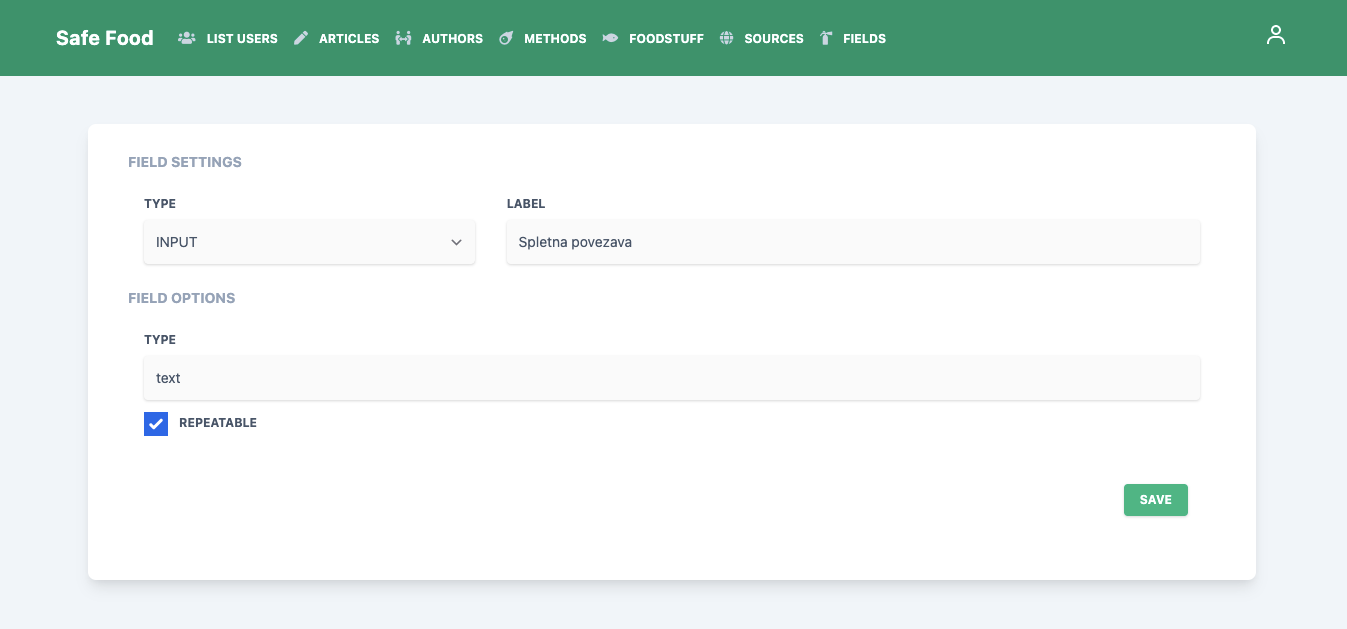
\includegraphics[width=1\textwidth]{slike/type_input.png}
\end{center}
\caption{ Definiranje vnosnega polja - input }
\label{type-input}
\end{figure}


\subsubsection{Izbirno polje}
Predstavlja podatek, ki je že vnaprej definiran in ga je mogoče izbrati. Izbirno polje je lahko definirano z ze v naprej dolocenimi vrednistmi, lahko pa se vrednosti dodaja sproti, medtem ko se vnasa podatke. Omogoca tudi iskanje po podatkih, in izbiranje vec le teh.
\begin{description}
     \item[taggable:] omogoca dodajanje novih vrednosti med samim urejanjem
     \item[multiple:] omogoca izbiro vec kot ene vrednosti
     \item[searchable:] omogoca iskanje po vnesenih vrednostih
 \end{description}

\begin{figure}[h]
\begin{center}
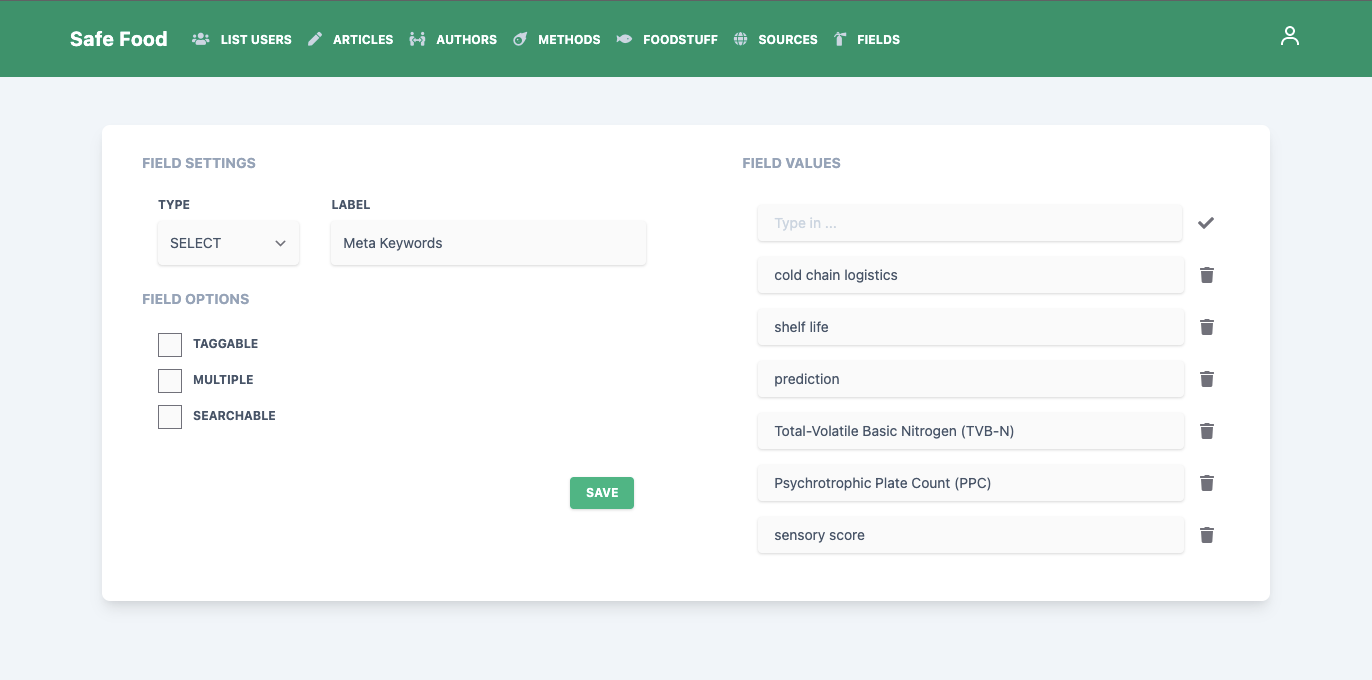
\includegraphics[width=1\textwidth]{slike/type_select.png}
\end{center}
\caption{ Definiranje vnosnega polja - select }
\label{type-select}
\end{figure}


\subsubsection{Izbirno polje - checkbox}
Predstavlja podatek, ki ga je mogoce izbrati (obkljukati) iz med prej definirah vrednosti. 

\begin{figure}[h]
\begin{center}
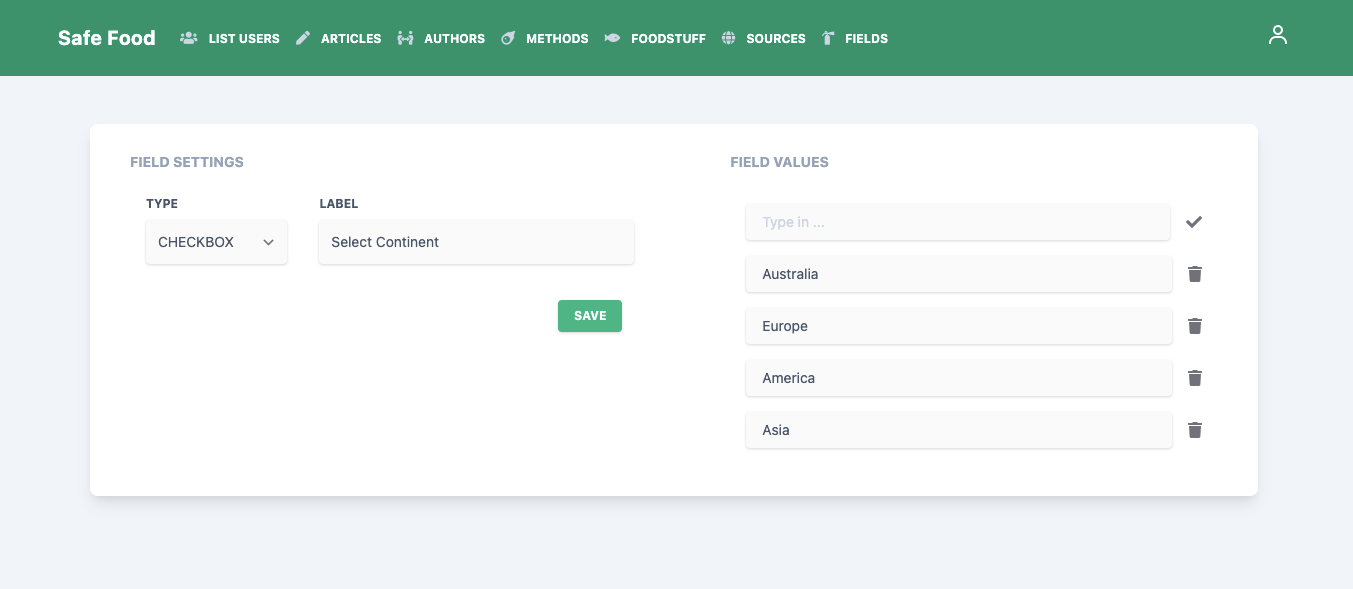
\includegraphics[width=1\textwidth]{slike/type_checkbox.png}
\end{center}
\caption{ Definiranje vnosnega polja - checkbox }
\label{type-checkbox}
\end{figure}


\subsubsection{Nalaganje datoteke}
Komponenta nam omogoca nalaganje datoteke za posamezno publicitacijo.

\begin{figure}[h]
\begin{center}

\includegraphics[width=1\textwidth]{slike/upload_file_zone.png}

\includegraphics[width=1\textwidth]{slike/upload_file_list.png}
\end{center}
\caption{ Prikaz graficnega vmestnika za nalaganje datotek }
\label{type-checkbox}
\end{figure}

\subsubsection{Polje za izbiranje casovnega podatka (datum)}
Predstavlja podatek, ki ga je mogoce izbrati (obkljukati) iz med prej definirah vrednosti. 

(https://day.js.org/en/)
Day.js je minimalistična knjižnica JavaScript, ki razčlenjuje, preverja, manipulira in prikazuje datume in ure za sodobne brskalnike z API-jem, ki je večinoma združljiv z Moment.js.
\begin{figure}[h]
\begin{center}
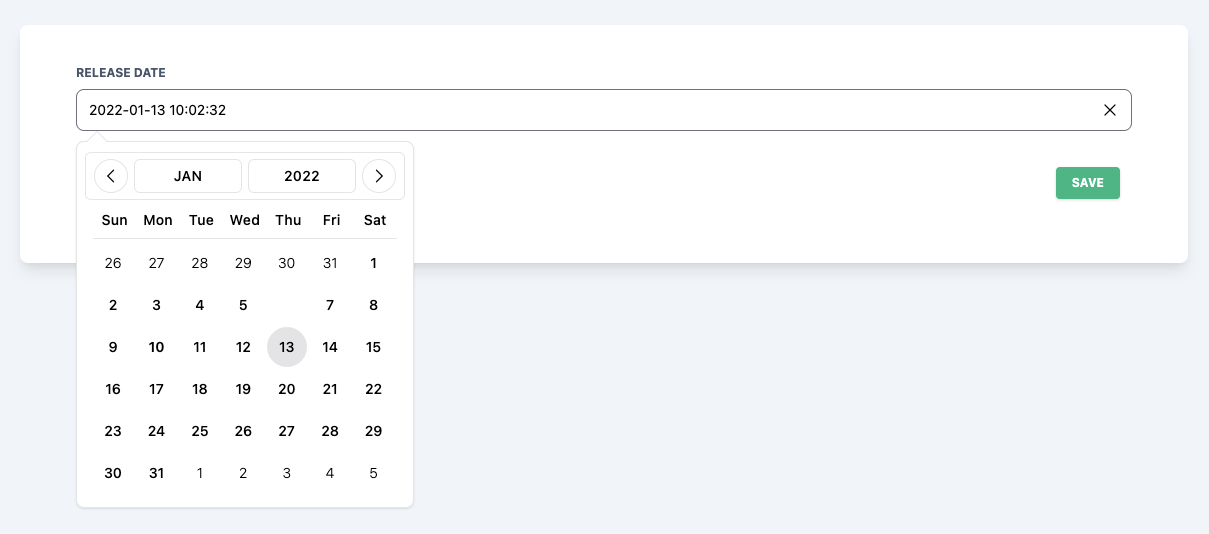
\includegraphics[width=1\textwidth]{slike/type_date.png}
\end{center}
\caption{ Prikaz graficnega vmestnika za izbiranje datuma }
\label{type-checkbox}
\end{figure}


\section{Iskanje objav}
\label{filters-page}
Vse vnešene publikacije so uporabniku prijazno prikazane na eni strani. Uporabnik ima možnost uporabe številnih filtrov, in s tem hitreje najde publikacijo, ki jo išče. Iskanje je omogočeno po vseh možnih podatkih, vnesenih za posamezno publikacijo. 

Stran je razdeljena na dva dela. Na levem delu strani so uporabniku na voljo filtri, katere lahko uporabi za iskanje po publikacijah, na desnem delu strani pa se uporabiku te publikacije prikažejo. 

Uporaba filtrov je enostavna. Na levem delu so izpisani vsi podatki, po katerih je mogoče iskati. Ob kliku na filter, se prikaže nabor vrednosti, katere lahko uporabik izbera, in s tem vklopi ali izklopi filter. V zgornjem delu strani je na voljo tudi iskanje po tekstovnem nizu besed, kjer uporabnik vnese iskan niz, in glede na niz se izvede filtracija.

\begin{figure}[h]
\begin{center}
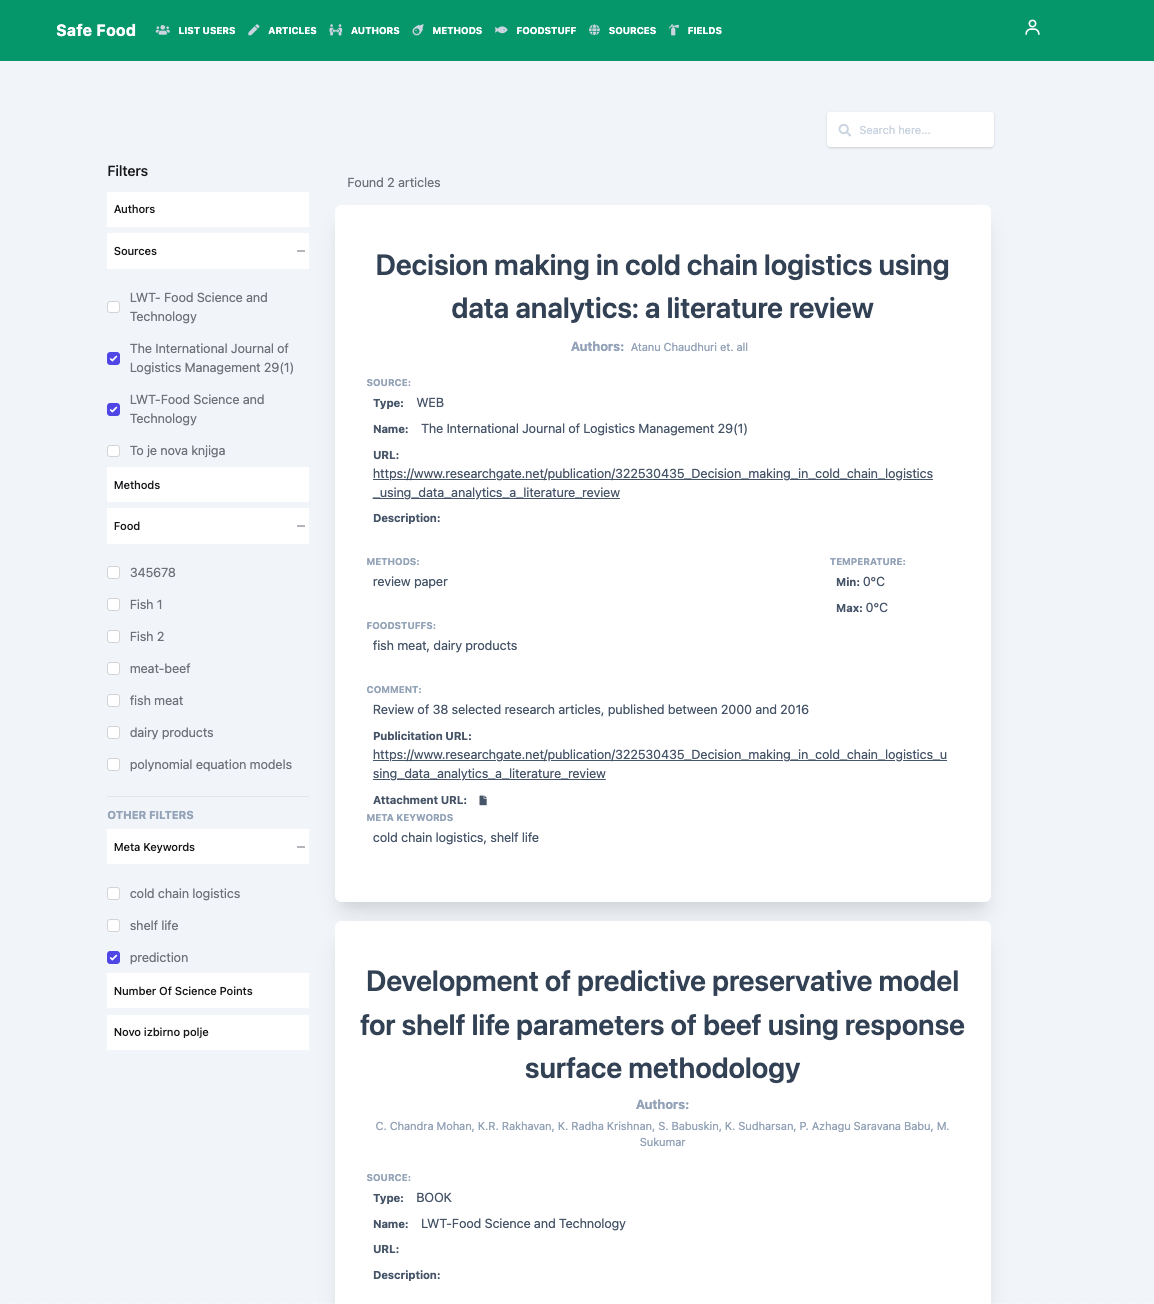
\includegraphics[width=1\textwidth]{slike/search.png}
\end{center}
\caption{ Prikaz uporabe filtrov }
\label{type-checkbox}
\end{figure}



\subsection{Problem s poizvedbo N+1}
Težava s poizvedbo N+1 se zgodi, ko je okvir za dostop do podatkov izvedel N dodatnih stavkov SQL, da bi pridobil iste podatke, ki bi jih bilo mogoče pridobiti pri izvajanju primarne poizvedbe SQL.

Večja kot je vrednost N, več poizvedb bo izvedenih, večji je vpliv na zmogljivost. In za razliko od dnevnika počasnih poizvedb, ki vam lahko pomaga pri iskanju počasnih poizvedb, težava N+1 ne bo opazna, ker se vsaka posamezna dodatna poizvedba izvaja dovolj hitro, da ne sproži dnevnika počasnih poizvedb.

Težava je pri izvajanju velikega števila dodatnih poizvedb, ki na splošno zahtevajo dovolj časa, da upočasnijo odzivni čas.


\chapter{Sklepne ugotovitve}
S projektom smo se naučili novih tehnologij in dela z mikrostoritvami. 

% \newpage %dodaj po potrebi, da bo številka strani za Literaturo v Kazalu pravilna!
% \\
\clearpage
\addcontentsline{toc}{chapter}{Literatura}
\bibliographystyle{plain}
\bibliography{diploma}


\end{document}

